\chapter{Background}
\label{ch:background}

This chapter will first go through the theoretical background needed to understand this thesis. This includes: the filtering metrics used to judge the quality of individual images, evaluation metrics to judge how those filtering metrics perform on a whole dataset of images, diffusion models, Bayesian machine learning and the Laplace approximation.
Additionally, practical and theoretical issues will be highlighted and linked to their consequences and solutions in later chapters.

\section{Inception Based Metrics}
\label{sec:inception_metrics}

In this section, we define the FID \parencite{heusel_gans_2018}, Precision, Recall, Realism \parencite{kynkaanniemi_improved_2019} and Rarity \parencite{han_rarity_2022} metrics. All of these operate in a shared feature space: each image (real or generated) is embedded by a pretrained \texttt{Inception-v3} network, yielding a feature vector $\phi$. We write $\boldsymbol{\Phi}_r = \{\phi_r^i\}$ and $\boldsymbol{\Phi}_g = \{\phi_g^i\}$ for the real and generated embedded feature sets respectively. For later definitions that can take either the real or generated feature set, we use $\boldsymbol{\Phi} \in \{\boldsymbol{\Phi}_r, \boldsymbol{\Phi}_g\}$.

We will first go through the batch scale\footnote{Batch scale refers to metrics that need a whole (large) dataset of generated samples to be computed on.} metrics \acs{FPR} (FID, Precision and Recall) aimed to evaluate the ``quality'' of the generated dataset compared to the real dataset.
We first define the simplest metric: the \acs{FID} from \cite{heusel_gans_2018} which relies on fitting a multivariate Gaussian to the generated and real datasets. Then we introduce two slightly more complex metrics: the ``improved'' Precision and Recall as presented in \cite{kynkaanniemi_improved_2019} which rely on a k-NN manifold approximation.

We finally define the individual\footnote{Opposite of batch scale, those metrics evaluate a single sample from the generated dataset which opens the door to filtering by assigning a score per sample.} samples metrics: Realism \parencite{kynkaanniemi_improved_2019} and Rarity \parencite{han_rarity_2022} that will be used as baseline to filter the samples and compare with Generative Uncertainty on the \acs{FPR} metrics. Filtering metrics are used to create subsets $\boldsymbol\Phi_f \subseteq \boldsymbol\Phi_g$ that only keep the $N$ best samples with respect to that filtering metric.

\begin{tcolorbox}[colback=orange!10!white,colframe=orange!50!black,sharp corners]
In this thesis, we use the \texttt{Inception-v3} model to match what was done in \cite{jazbec_generative_2025} while the actual paper introducing the Precision, Recall and Realism metrics \parencite{kynkaanniemi_improved_2019} uses a VGG-16 classifier layer instead. \cite{kynkaanniemi_improved_2019} however also tested their metric with \texttt{Inception-v3} and it lead to very similar results in their experiments.
\end{tcolorbox}

\subsection{Fréchet Inception Distance (FID)}
\label{subsec:fid}

The FID \cite{heusel_gans_2018} compares the \emph{statistical distributions} of
real and generated feature vectors by fitting a multivariate Gaussian to each
dataset $\boldsymbol{\Phi}_r,\boldsymbol{\Phi}_g$ and computing the squared Fréchet distance between them:
%
\begin{equation}
  \label{eq:fid}
  \mathrm{FID}
  \;=\;
  \|\mu_{r} - \mu_{g}\|_{2}^{2}
  \;+\;
  \operatorname{Tr}\!\left(
    \Sigma_{r} + \Sigma_{g}
    - 2\bigl(\Sigma_{r}^{1/2}\Sigma_{g}\Sigma_{r}^{1/2}\bigr)^{1/2}
  \right),
\end{equation}
%
where $(\mu_{r}, \Sigma_{r})$ and $(\mu_{g}, \Sigma_{g})$ are the empirical
means and covariances of $\boldsymbol{\Phi}_{r}$ and $\boldsymbol{\Phi}_{g}$.
The first term penalises a shift in mean appearance; the second penalises
any mismatch in spread and correlation, capturing both mode collapse (too
narrow) and over-dispersion (too broad).
Lower is better.
 
% Despite its widespread adoption, FID has notable structural weaknesses
% \cite{jayasumana_rethinking_2024}: the Gaussian assumption is rarely satisfied in
% practice, Inception-v3 features poorly represent the semantic content of
% modern generative models, and the estimator is statistically biased with
% poor sample complexity, making cross-paper comparisons unreliable.
% These limitations motivate the HPSv3 supplementary metric (\autoref{ch:hpsv3}).

\begin{tcolorbox}[colback=orange!10!white,colframe=orange!50!black,sharp corners]
Despite its widespread adoption, FID suffers from notable structural weaknesses \parencite{jayasumana_rethinking_2024} that will be described among other issues in \autoref{sub:problems_inception}.
\end{tcolorbox}

\subsection{k-NN Manifold Estimate}

Before going on to define the Precision, Recall, Realism and Rarity metrics, we need to properly define what the k-NN Manifold Approximation is.

\begin{tcolorbox}[colback=gray!10!white,colframe=gray!50!black,sharp corners]
The intuitive idea here is that each point in the embedding space $\phi \in \boldsymbol{\Phi}$ is assigned a ball for which the radius is defined by the distance between $\phi$ and its k-th closest neighbor. Taking the union of all those balls gives an approximation of the manifold defined by the real or generated dataset (\autoref{fig:bg_knn_manifold} for an intuitive visualization).
\end{tcolorbox}

\begin{figure}[!htbp]
    \centering
    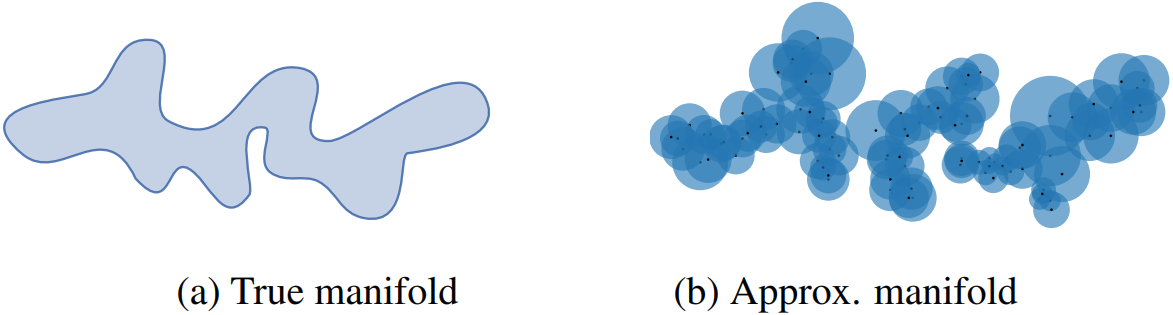
\includegraphics[width=0.9\linewidth]{figures/background/knn_manifold.png}
    \caption{Taken from \cite{kynkaanniemi_improved_2019} (a) An example manifold in a feature space. 
    (b) Estimate of the manifold obtained by sampling a set of points and surrounding each with a hypersphere that reaches its $k$-th nearest neighbor, defining $\mathcal{M}_k$.}
    \label{fig:bg_knn_manifold}
\end{figure} 

More rigorously, we define the radius of the hypersphere surrounding each feature vector $\phi^i \in \boldsymbol{\Phi}$ as  $||\phi^i - \mathrm{NN}_k(\phi^i, \boldsymbol{\Phi})||_2$ where $\mathrm{NN}_k(\phi^i, \boldsymbol{\Phi})$ is the k-th nearest vector to $\phi^i$ in $\boldsymbol{\Phi}$. The ball is then defined as:
\begin{align}
  B_{k}(\phi^{i},\boldsymbol{\Phi})
  &= \bigl\{\phi \mid \|\phi - \phi^{i}\|_{2} \le ||\phi^i - \mathrm{NN}_{k}(\phi^{i},\boldsymbol{\Phi})||_2\bigr\}. \label{eq:knn_ball_cond}
\end{align}

And finally, the approximation of the underlying manifold of $\boldsymbol{\Phi}$ is constructed as:
\begin{align}
  \label{eq:manifold}
  \mathcal{M}_{k}(\boldsymbol{\Phi}) &= \bigcup_{\phi^{i} \in \boldsymbol{\Phi}} B_{k}(\phi^{i},\boldsymbol{\Phi}),
\end{align}

% (\autoref{fig:bg_knn_manifold} \cite{kynkaanniemi_improved_2019}): each feature vector $\phi_i \in \Phi$ is

Lastly, we define a helper function for the membership of a given sample $\phi$ to an approximated manifold $\mathcal{M}_k(\boldsymbol{\Phi})$
\begin{align}
f(\phi, \boldsymbol{\Phi}) &= 
    \begin{cases} 
      0 & \phi \not \in \mathcal{M}_k(\boldsymbol{\Phi})\\
      1 & \phi \in \mathcal{M}_k(\boldsymbol{\Phi})
\end{cases}
\label{eq:f_helper_func_mk}
\end{align}

\begin{tcolorbox}[colback=gray!10!white,colframe=gray!50!black,sharp corners]
Intuitively, dense regions of the distribution produce many small, tightly packed balls;
sparse regions produce large, widely spaced ones.
A point $\phi$ is considered to lie \emph{inside} the manifold if it
falls within at least one of these balls $B_k$, i.e.\ if there exists some anchor
$\phi^i \in \boldsymbol{\Phi}$ such that $\|\phi - \phi^i\|_2 \le ||\phi^i - \mathrm{NN}_k(\phi^i, \boldsymbol{\Phi})||_2$.
\end{tcolorbox}


The choice of the neighborhood size $k$ represents a compromise between fully covering the underlying manifold and overestimating its volume. Empirical evaluations across various datasets establish $k=3$ as a robust default, as it generally avoids saturating precision and recall scores while keeping the proportion of out-of-manifold samples well below 30\% \cite{kynkaanniemi_improved_2019,han_rarity_2022}. Consequently, we adopt $k=3$ alongside standard sample sizes of $|\boldsymbol{\Phi}_r| = 50{,}000$. 

\begin{tcolorbox}[colback=orange!10!white,colframe=orange!50!black,sharp corners]
Following \cite{kynkaanniemi_improved_2019}, the size of the generated dataset should also be $|\boldsymbol{\Phi}_g|= 50{,}000$. In \cite{jazbec_generative_2025} however, when testing the impact of filtering the generated dataset, they start with $|\boldsymbol{\Phi}_g| = 12{,}000$ and end up at $|\boldsymbol{\Phi}_f| = 6{,}000$ samples. We will go over the consequences of this in \autoref{sub:problems_inception}.
\end{tcolorbox}

\subsection{Precision and Recall}
\label{subsec:precision-recall}

\begin{figure}[!htbp]
    \centering
    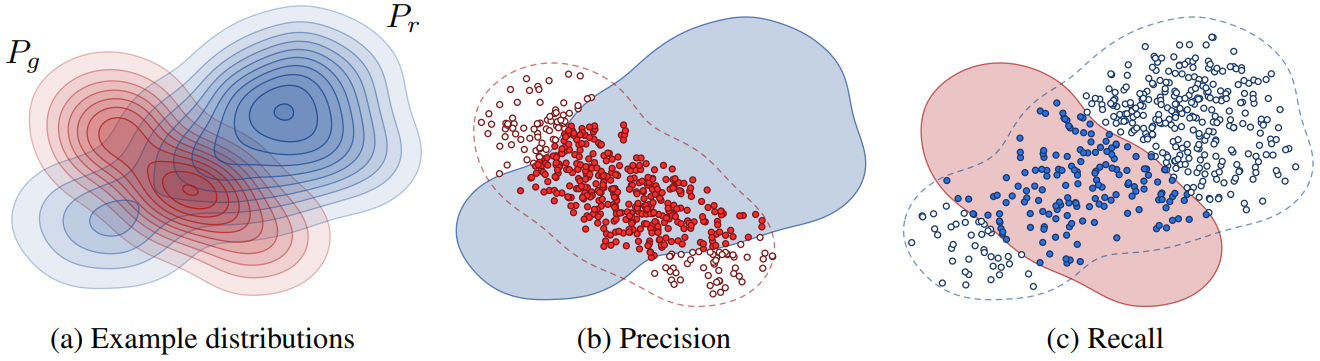
\includegraphics[width=0.9\linewidth]{figures/background/precision_recall.png}
    \caption{Taken from \cite{kynkaanniemi_improved_2019}: Definition of precision and recall for distributions. 
    (a) Denote the distribution of real images with $P_r$ (blue) and the distribution of generated images with $P_g$ (red). 
    (b) Precision is the probability that a random image from $P_g$ falls within the support of $P_r$. (c) Recall is the probability that a random image from $P_r$ falls within the support of $P_g$.}
    \label{fig:bg_precision_recall}
\end{figure}
 
FID conflates two independently important aspects of generation quality.
\emph{Precision} (fidelity) asks whether generated images look realistic;
\emph{recall} (diversity) asks whether the generated distribution covers the
full variety of real images.
A generator suffering from mode collapse can have high precision but low
recall; a generator producing noisy, incoherent samples that happen to span
the data space can have high recall but low precision.
\citet{kynkaanniemi_improved_2019} disentangle the two using the manifold estimator
$\mathcal{M}_k(\boldsymbol{\Phi})$:
%
\begin{align}
  \mathrm{Precision}(\boldsymbol{\Phi}_{r}, \boldsymbol{\Phi}_{g})
  &=
  \frac{1}{|\boldsymbol\Phi_{g}|}
  \sum_{\phi_{g}^{j} \in \boldsymbol\Phi_{g}}
  f\!\left(\phi_{g}^{j}, \boldsymbol\Phi_{r}\right), 
  \label{eq:precision}\\[4pt]
  \mathrm{Recall}(\boldsymbol\Phi_{r}, \boldsymbol\Phi_{g})
  &=
  \frac{1}{|\boldsymbol\Phi_{r}|}
  \sum_{\phi_{r}^{i} \in \boldsymbol\Phi_{r}}
  f\!\left(\phi_{r}^{i}, \boldsymbol\Phi_{g}\right).
  \label{eq:recall}
\end{align}
%
\begin{tcolorbox}[colback=gray!10!white,colframe=gray!50!black,sharp corners]
Precision counts the fraction of generated samples that fall inside the real
manifold (i.e.\ satisfy the $k$-NN ball condition \eqref{eq:knn_ball_cond}). Recall counts the fraction of real samples covered by the generated manifold.
\end{tcolorbox}

Both metrics make no distributional assumptions, in contrast to FID.

Precision and recall are not independent ($\indep$): retaining only the highest-quality generated images improves precision but shrinks the coverage of real modes, reducing recall.
% This trade-off is visible throughout our filtering experiments and mirrors the
% quality-diversity trade-off induced by classifier guidance \cite{dhariwal_diffusion_2021}.

\subsection{Realism Score}
% \label{sec:filtering-metrics}
\label{subsec:realism}

% The two non-uncertainty baselines we compare against are the realism and rarity scores \cite{kynkaanniemi_improved_2019,han_rarity_2022}.
% Both operate in a shared feature space: each image (real or generated) is
% embedded by a pretrained \texttt{Inception-v3} network, yielding
% a $2048$-dimensional feature vector $\phi$.
% We write $\Phi_{r} = \{\phi^{r}_{i}\}$ and $\Phi_{g} = \{\phi^{g}_{j}\}$
% for the real and generated feature sets respectively, and use
% $\mathrm{NN}_{k}(\phi, \Phi)$ to denote the $\ell_2$-distance from $\phi$
% to its $k$-th nearest neighbour in $\Phi$.

In the same paper as Precision and Recall, \cite{kynkaanniemi_improved_2019} introduce Realism, a metric that can be used to score individual samples by providing an estimate of how deeply a generated sample penetrates the real manifold by comparing the radius of a real neighborhood to the distance from
the generated sample to its center. Taking the maximum gives the deepest penetration. 

\begin{align}
    R = \mathrm{Realism}(\phi_g, \boldsymbol\Phi_r) &=
    \max_{\phi_r \in \boldsymbol\Phi_r^*}
    \left\{ \frac{||\phi_r - \mathrm{NN}_k(\phi_r, \boldsymbol{\Phi}_r)||_2}{||\phi_g-\phi_r||_2}\right\}
\end{align}

where $\boldsymbol\Phi_r^* \subseteq \boldsymbol\Phi_r$ is a filtered subset of real anchors defined below. 
The score gets bigger as the generated sample $\phi_g$ gets closer to $\mathcal{M}_k(\boldsymbol\Phi_r)$ until $R \ge 1$ at which point we have an equivalence with $f(\phi_g, \boldsymbol\Phi_r)$ \eqref{eq:f_helper_func_mk}: $f(\phi_g, \boldsymbol{\Phi}_r) = 1 \iff R(\phi_g, \boldsymbol{\Phi}_r) \ge 1$. 
The ratio $R$ can be seen as a continuous extension of the helper function $f$ \eqref{eq:f_helper_func_mk}.

Lastly, one flaw of the k-NN approximation is to assign large hyperspheres to points in sparse regions (low sample density). 
If a sample happens to fall in such a region, it can lead to a highly inaccurate score $R$. To fix this, instead of taking the $\max$ across all $\phi_r \in \boldsymbol{\Phi}_r$, we create a subset $\boldsymbol{\Phi}_r^*$ by taking $\boldsymbol{\Phi}_r$ and removing all $\phi_r$ that have a hypersphere of radius bigger than the median radius.

Regarding Precision and Recall, because it is unlikely that a sample falls in a low density region, even with larger hyperspheres, the proportion of samples affected by this is quite low. Therefore, Precision and Recall being evaluated on large populations of generated samples, do not need such precautions (according to \cite{kynkaanniemi_improved_2019}).

% \begin{equation}
%   \label{eq:realism}
%   \mathrm{realism}(\phi^{g}_{j})
%   \;=\;
%   \max_{\substack{\phi^{r}_{i} \in \Phi_{r} \\ \mathrm{NN}_{k}(\phi^{r}_{i},\Phi_{r}) \le m}}
%   \frac{\mathrm{NN}_{k}(\phi^{r}_{i},\Phi_{r})}
%        {\|\phi^{r}_{i} - \phi^{g}_{j}\|_{2}}.
% \end{equation}

% The ratio compares the radius of a real neighborhood to the distance from
% the generated sample to its centre; a value above $1$ means the sample
% falls inside that ball. Taking the maximum over real anchors selects the deepest penetration. 
% Crucially, to prevent massive, sparsely-located hyperspheres from yielding wildly inaccurate scores, the maximum is only taken over anchors whose hypersphere radius is smaller than the median radius $m$ of the real manifold \cite{kynkaanniemi_improved_2019}.
% We retain the $n$ generated images with the \emph{highest} realism scores.
 
\subsection{Rarity Score}
\label{subsec:rarity}

While realism was good at evaluating how close a generated image was to the real data manifold, it did so by rewarding images that stayed in safe, familiar territory.
The Rarity score \cite{han_rarity_2022} was introduced to explicitly evaluate the ``uncommonness'' of an individual generated image while still detecting and isolating \acs{OOD} (Out Of Distribution) samples, thereby rewarding models that can generate those edge cases without producing \acs{OOD}.

% rewarding models that can successfully generate these edge cases without producing \acs{OOD} (out-of-distribution) samples.
% The rarity score~\cite{han_rarity_2022} quantifies the uncommonness of a generated sample based on the density of the real data distribution. It is defined as the minimum radius among the real $k$-NN spheres that contain the given fake sample:
%
% \begin{align}
%   \label{eq:rarity}
%   \mathrm{Rarity}(\phi_{g})
%   &=
%   \min_{\substack{\phi^{r}_{i} \in \Phi_{r} \\ \phi^{g}_{j} \in B_{k}(\phi^{r}_{i},\Phi_{r})}}
%   \mathrm{NN}_{k}(\phi^{r}_{i},\Phi_{r}).
% \end{align}
For a generated sample $\phi_g^j$, we take every ball $B_k$ penetrated by $\phi_g^j$ and take the smallest ball radius as Rarity score. The bigger the radius, the less dense the region of the manifold which is what rarity tries to measure, additionally, if $\phi_g^j$ does not penetrate any ball, we consider it \acs{OOD}. Here is the mathematical formulation:

\begin{equation}
  \mathrm{Rarity}(\phi_{g}^j, \boldsymbol{\Phi}_r)=
  \begin{cases}
  \min\limits_{\substack{\phi_{r}^{i} \in \boldsymbol\Phi_{r} \\ \mathrm{s.t.} \;  \phi_{g}^{j} \in B_{k}(\phi_{r}^{i},\boldsymbol\Phi_{r})}}
  ||\phi_r^i - \mathrm{NN}_{k}(\phi_{r}^{i},\boldsymbol\Phi_{r})||_2 & \exists \phi^i_r\\
  \mathrm{O.O.D.} & \not\exists \phi_r^i
  \end{cases}
  \label{eq:rarity}
\end{equation}
%


% By taking the minimum of the radius of the hyper-sphere, the metric avoids overestimating the sparsity of a generated sample that happens to fall into multiple overlapping spheres. A high rarity score indicates that the sample resides in a low-density region of the real manifold, exhibiting unique or extraordinary characteristics. Conversely, a low rarity score indicates a highly typical, common image \cite{han_rarity_2022}. Because the fidelity of samples completely outside the real manifold cannot be guaranteed, their rarity scores are undefined, and they are discarded. Depending on the desired output, one can retain the $n$ generated images with the \emph{highest} rarity scores to sample high-diversity generation, or the \emph{lowest} to ensure typicality.
 
Realism and rarity are thus complementary: realism rewards proximity to the real manifold, while rarity rewards distance from its high-density core. 
In \cite{jazbec_generative_2025} however, they aim to remove artifacts out of the dataset. They hypothesize that those artifacts are located in the lower density regions meaning they use the rarity score for filtering by keeping the images with \textbf{lowest} rarity.

\subsection{Problems with this Framework}
\label{sub:problems_inception}

Here we list and explain all identified problems ranging from the metrics themselves to how they were computed in \cite{jazbec_generative_2025}. This helps to motivate \autoref{ch:hpsv3}, where we define a new metric that we believe is not affected by those problems.

\paragraph{Inception-V3 Encoder}
First and foremost, all of these metrics rely on the same embedding space provided by the \texttt{Inception-v3} encoder and this leads to the following issues:
\begin{itemize}
    \item The FID metric has been criticized for contradicting human judgement, partly attributing the problem to the \texttt{Inception-v3} encoder \parencite{jayasumana_rethinking_2024}; this issue would therefore affect all other Inception-based metrics.
    \item Using the same encoder for both the Realism and Rarity filtering metric and the \acs{FPR} evaluation metrics leads to a bias that is likely disadvantageous for methods that do not use the \texttt{Inception-v3} encoder, such as \cite{jazbec_generative_2025} Generative Uncertainty (\acs{GU}).
\end{itemize}

% \begin{enumerate}
    % \item Approximating the both the real and generated image distribution by a multivariate gaussian is provably incorrect \parencite{jayasumana_rethinking_2024}.
    % \item The FID computation requires the computation of two covariance matrix $\Sigma_r, \Sigma_g$ of size $2048 \times 2048$ which lead to poor sample efficiency: see \autoref{fig:bg_cmmd_vs_fid}.  \label{enum:fid_critique_sample_efficiency}
    % Inception-v3 features poorly represent the semantic content of modern generative models, and the estimator is statistically biased with poor sample complexity. Because this bias depends on the model being evaluated, it can lead to different rankings of the models based on sample size. In the context of this thesis, these limitations make cross-paper comparisons unreliable and motivate the use of the HPSv3 supplementary metric (Chapter 7).
% \end{enumerate}

% \begin{figure}[!htbp]
%     \centering
%     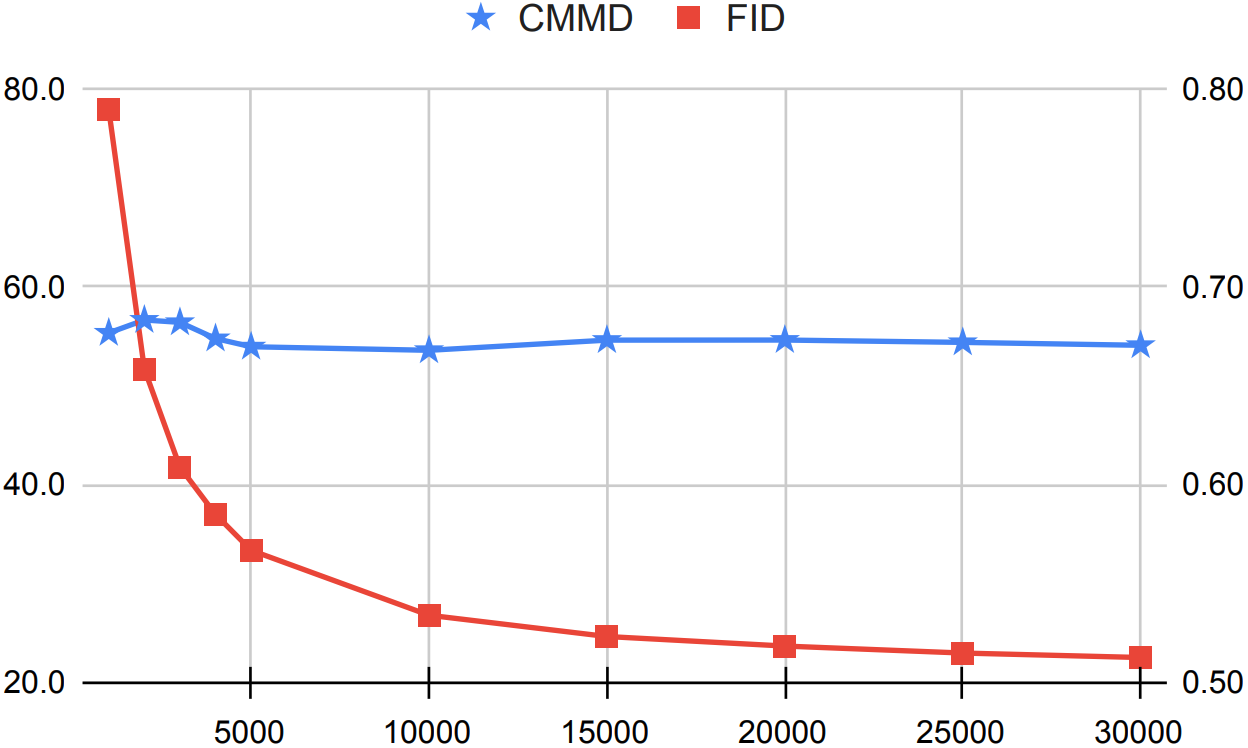
\includegraphics[width=0.7\linewidth]{figures/background/cmmd_vs_fid.png}
%     \caption{Taken from \cite{jayasumana_rethinking_2024}. The relation between FID and the sample size used to compute the FID. We expect a metric to independent from the sample size, FID clearly is not. CMMD is \cite{jayasumana_rethinking_2024} attempt at fixing the flaws from FID.}
%     \label{fig:bg_cmmd_vs_fid}
% \end{figure}

% \paragraph{Filtered Dataset Size}

% As noted before, instead of using a symetric number of samples $|\boldsymbol{\Phi}_r|=|\boldsymbol{\Phi}_g|=50{,}000$, \cite{jazbec_generative_2025} uses $|\boldsymbol{\Phi}_r| = 50{,}000$ for the real dataset but only uses from $|\boldsymbol{\Phi}_g| = 12{,}000$ to $|\boldsymbol{\Phi}_f| = 6{,}000$ for generated/filtered datasets. The consequences for this include:

% \begin{enumerate}
%     \item Similarly as with the FID: Precision and Recall are influenced by the sample size.  (\autoref{fig:fpr_sample_size}):
%     \begin{itemize}
%         \item Precision is the least affected because it looks at 
%     \end{itemize}
% \end{enumerate}
% \begin{enumerate}
%     \item With $|\boldsymbol{\Phi}_r| = 50{,}000$ reference points but only $|\boldsymbol{\Phi}_f| = 6{,}000$, the density of the reference manifold $\mathcal{M}_k(\boldsymbol{\Phi_r})$ will be artificially much higher than the generated manifold $\mathcal{M}_k(\boldsymbol{\Phi}_f)$. This severely biases the Recall score, as the metric will underestimate the volume of the generated manifold simply because it is sparsely sampled.
% \end{enumerate}
\paragraph{Effect of using a small sample size}

As highlighted before, instead of the recommended $|\boldsymbol{\Phi}_r| = |\boldsymbol{\Phi}_g| = 50{,}000$, \cite{jazbec_generative_2025} and by extension, this thesis, uses $|\boldsymbol\Phi_g| = 12{,}000$ and $|\boldsymbol\Phi_f| \in \left[6000,\dots, 12000\right]$. There are two effects of sample size that we will study here:
The sample size itself $|\boldsymbol{\Phi}|$ and the asymmetry of using a sample size $|\boldsymbol{\Phi}_g| \not= |\boldsymbol\Phi_r|$.

The effect of sample size $|\boldsymbol\Phi|$ has been studied for both FID \parencite{jayasumana_rethinking_2024} and Precision, Recall \parencite{kynkaanniemi_improved_2019}.

\begin{enumerate}
    % \item \boldsymbol{FID}: \cite{jayasumana_rethinking_2024} highlights the 
    \item The FID computation requires the computation of two covariance matrices $\Sigma_r, \Sigma_g$ of size $2048 \times 2048$, which leads to poor sample efficiency\footnote{FID needs a very large sample size to become stable with respect to variations of the sample size} \parencite{jayasumana_rethinking_2024}. \label{enum:fid_critique_sample_efficiency}
    \item Because Precision and Recall rely on the k-NN manifold approximation, having a smaller dataset size $|\boldsymbol\Phi|$ implies a lower density of points across the semantic space making the distance to the $k$-th neighbor bigger and therefore the hypersphere associated to each point bigger, it becomes easier for points of each either $\boldsymbol\Phi_{r,g}$ to fall into the manifold associated to the other distribution $\mathcal{M}_k(\boldsymbol\Phi_{g,r})$, artificially increasing the Precision and Recall scores.
\end{enumerate}

\begin{figure}[!htbp]
    \centering
    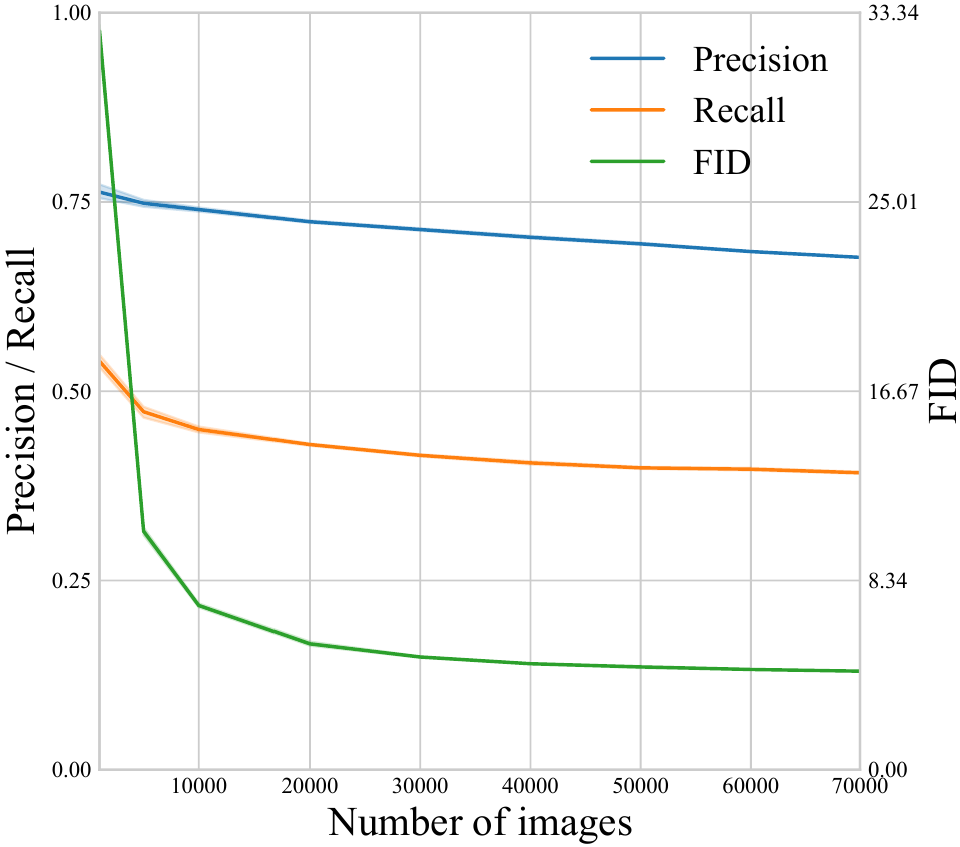
\includegraphics[width=0.6\linewidth]{figures/background/fpr_sample_size.png}
    \caption{Taken from \cite{kynkaanniemi_improved_2019}, We already knew about the effect of reducing the sample size on the FID. This figure also shows what happens to Precision and Recall. FID is clearly the most affected, followed by Recall and Precision}
    \label{fig:fpr_sample_size}
\end{figure}

\autoref{fig:fpr_sample_size} illustrates this phenomenon in \cite{kynkaanniemi_improved_2019}'s experimental setup. When looking into the range $[6000,\dots,12000]$ (to match \cite{jazbec_generative_2025}) FID is by far the most affected. Recall is also affected in a visible way, while Precision appears to be significantly more stable.

One plausible explanation for this stems from the spatial differences between $\mathcal{M}_k(\boldsymbol\Phi_r)$ and $\mathcal{M}_k(\boldsymbol\Phi_g)$. 

Recall evaluates whether real images fall within the generated manifold.
Generative models generally cover a smaller fraction of the true data distribution\footnote{This is also a motivation for the creation of metrics such as Precision and Recall}. Because generated samples are packed into a smaller subset of the feature space, lowering the sample size forces the $k$-NN boundaries of these dense clusters to grow. Since this generated manifold sits within the broader real distribution, expanding its boundaries rapidly engulfs peripheral real points, causing Recall to spike artificially. 

In contrast, Precision evaluates whether generated images fall within the real manifold. Because models tend to generate samples in safe, well-represented regions, most generated points already reside deep inside the real distribution. Therefore, when the broad real manifold expands outward into empty space due to sparsity, it captures very few new generated points, resulting in a much flatter growth curve for Precision.

In \cite{jazbec_generative_2025} however, we fix the size of the real dataset $|\boldsymbol{\Phi}_r| = 50{,}000$ and vary the size of the generated dataset $N = |\boldsymbol\Phi_f| \in [6000,\dots,12000]$. This asymmetry makes precision even less sensitive to $N$ because $\mathcal{M}_k(\boldsymbol\Phi_r)$ is fixed: only the number of generated points changes and most of them reside in the real distribution. Recall however grows even more from it because it measures how well the huge $50{,}000$-point dataset fits into $\mathcal{M}_k(\boldsymbol\Phi_g)$, whose hyperspheres keep growing around the clusters.

\begin{tcolorbox}[colback=red!10!white,colframe=red!50!black,sharp corners]
We will come back to this issue in \autoref{ch:reproduce_adm} to both illustrate its effect it in practice (with the \cite{jazbec_generative_2025} experiment) and show how take it into account when evaluating filtering methods.
\end{tcolorbox}


% Generative models, often suffer from missed modes or reduced variation, meaning they generally cover a smaller fraction of the true data distribution. This is in fact the whole premise \cite{kynkaanniemi_improved_2019} and what Precision and Recall tries to measure.

% Because the generated manifold has less intrinsic variation and covers less total volume, taking a small number of samples from it causes its $k$-NN hyperspheres to inflate drastically to bridge the gaps between the generated points. Therefore, the estimated volume of the generated manifold (used to calculate Recall) expands proportionally more aggressively than the broad real manifold (used to calculate Precision).

% As the generated manifold rapidly inflates, it suddenly swallows up real data points that it would normally miss, causing that steeper artificial spike in the Recall score.
% \begin{itemize}
%     \item The nature of the real manifold drives Precision. The real dataset (like ImageNet) is incredibly diverse, and most likely spans a vast volume in the encoder's latent space. When we sparsely sample this vast space, the data points are extremely far apart. To find the $k$-th nearest neighbor, the hyperspheres drawn around these real points expand massively. Because Precision asks, ``Does the generated points fall inside the real spheres?'', the scale of the real spheres makes it easier for them to capture more generated points. This causes Precision to artificially rise.
%     \item The nature of the generated manifold drives Recall. Generative models likely tend to concentrate around safer, higher-density regions and. The generated manifold would therefore naturally occupy a smaller, less diverse volume. This leads to the hyperspheres remaining smaller for longer as we reduce the number of generated samples. Recall asks ``Does the real points fall inside the generated points spheres?'', the real points stay well scattered accross the whole space and the shape of the approximated generated dataset manifold does not change much so the metric remains somewhat flat.
% \end{itemize}


\paragraph{FID Specific Critique}
The Gaussian assumption in FID has also been critiqued \parencite{jayasumana_rethinking_2024}: ``approximating both the real and generated image distribution by a multivariate Gaussian is provably incorrect''.

\paragraph{Batch Scale Metrics}

The fact that \acs{FPR} metrics need large \textit{batches} of generated data for them to be meaningful makes their evaluation extremely expensive. In \cite{jazbec_generative_2025} for instance we use 12032 images generated by $M+1=6$ models which takes around 20 hours of compute on a \texttt{Tesla A100}. 
This motivates the need for an evaluation metric that can be computed \textit{per-image}. One could use Realism and Rarity for that but we are already using those metrics as filtering baselines and using Realism and Rarity would not fix most of the issues highlighted above.
 
% ============================================================
 
% \section{Evaluation Metrics}
% \label{sec:eval-metrics}
 
% All three evaluation metrics below operate in the same Inception-v3 feature
% space defined above.
% ; the HPSv3 metric (Chapter~\ref{ch:semantic}) provides an
% independent, human-preference-based view.
 
 \paragraph{Conclusion}

 In short:
\begin{itemize}
    \item The \texttt{Inception-v3} encoder does not suit our needs \parencite{jayasumana_rethinking_2024}.
    \item FID contradicts human judgement \parencite{jayasumana_rethinking_2024}.
    \item Using the same encoder for both \acs{FPR} and the Realism/Rarity baselines is disadvantageous for methods that do not use the \texttt{Inception-v3} encoder, such as Generative Uncertainty.
    \item Using small and asymmetric dataset sizes causes artificial inflation of the \acs{FPR} metrics when filtering, leading to false conclusions if not accounted for.
    \item \acs{FPR} metrics require huge generated datasets, making them extremely expensive to compute.
\end{itemize}

In light of those issues, we've decided to keep \cite{jazbec_generative_2025} experiments setup as it is and instead add a brand new metric that will serve as an ``oracle'' of judging if an image is realistic or not. For this, we will use a pretrained model that outputs a human preference score (\autoref{ch:hpsv3}).

\section{Diffusion Models}
\label{sec:bg_diffusion}

Diffusion models are a class of deep generative models first introduced from the perspective of nonequilibrium thermodynamics \parencite{sohl2015thermo}, and later shown to produce image samples competitive with, or superior to, generative adversarial networks \parencite{ho_denoising_2020, dhariwal_diffusion_2021}. They learn to synthesize high-quality data by progressively transporting a simple prior distribution to a complex data distribution. This thesis works within the classical discrete-time formulation of this idea \parencite{ho_denoising_2020, song_denoising_2022}, which we build up over the following subsections. The framework also admits continuous-time and flow-based generalisations, which we summarise briefly in \autoref{subsec:bg_continuous}.

\subsection{Formal Setup}
Suppose we are given a training dataset $\mathcal{D} = \{x_n\}_{n=1}^N$ drawn from a true underlying data distribution $p_{\mathrm{data}}(x)$.
Depending on the domain, the data $x \in \mathcal{X}$ can take various mathematical forms. For example, in the case of natural images, $x$ is a high-dimensional tensor $x \in \mathbb{R}^{H \times W \times C}$. In this thesis we simply write $x \in \mathbb{R}^D$.

The ultimate goal of generative modeling is to define a generator function, $g_{\theta} : \mathcal{Z} \rightarrow \mathcal{X}$ parameterized by model weights $\theta \in \mathbb{R}^{P}$, which maps an initial noise variable $z \in \mathcal{Z}$ drawn from a prior distribution $z \sim p_{\mathrm{init}}(z)$ (typically a standard Gaussian $\mathcal{N}(0, I)$) to a new data sample $\hat{x}$. However, unlike other deep generative models such as variational autoencoders or generative adversarial networks that attempt to learn this complex mapping in a single leap, diffusion models decompose it into a progressive, step-by-step process \parencite{ho_denoising_2020}.

Conceptually, this process consists of two distinct phases. First, a forward process systematically destroys the structure of the data by adding random noise until it becomes pure noise (matching $p_{\mathrm{init}}(z)$). Secondly, a reverse process trains a neural network to systematically remove that noise, effectively learning how to generate data from pure noise. This framework is versatile enough to be applied to varying tasks, 
from a simple 2D synthetic dataset featuring 25 distinct Gaussian modes (e.g., the Toy experiment in \autoref{ch:reproduce_toy}), to high-dimensional datasets like ImageNet $128 \times 128$ using advanced architectures such as the \acf{ADM} (e.g., the \acs{ADM} experiment in \autoref{ch:reproduce_adm}) \cite{jazbec_generative_2025}.

\begin{figure}[!htbp]
    \centering
    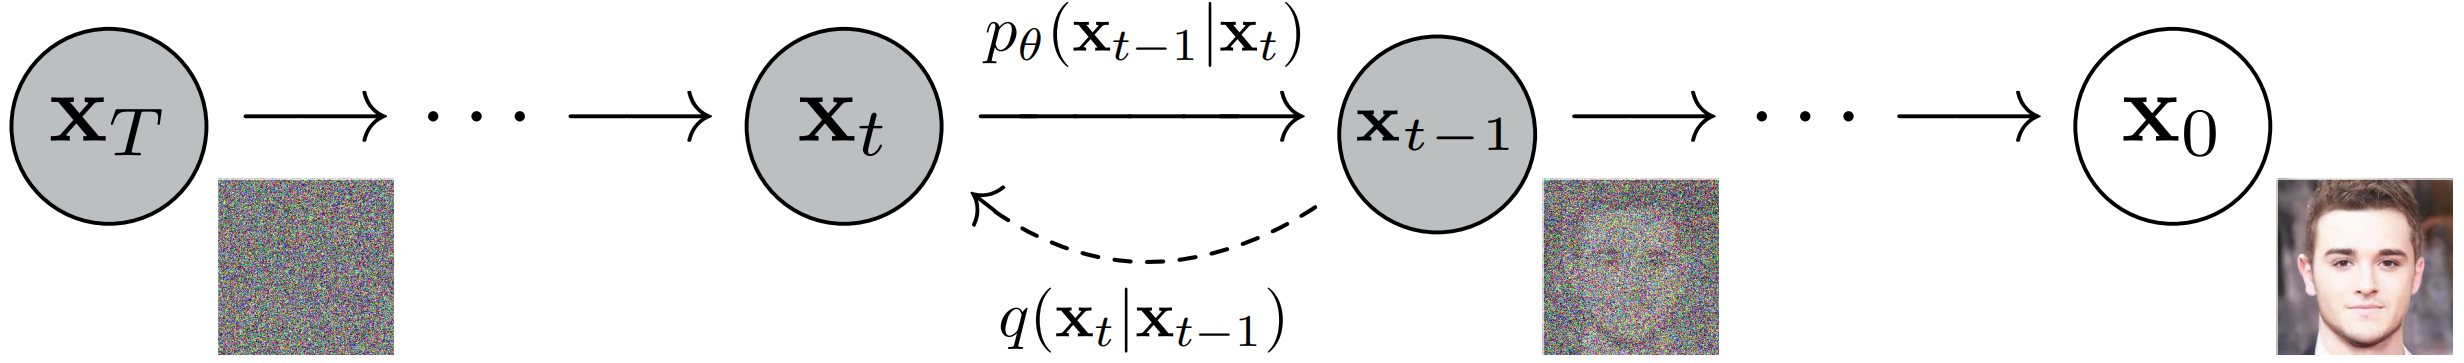
\includegraphics[width=0.9\linewidth]{figures/theory/diffusion_markov.png}
    \caption{Illustration from \cite{ho_denoising_2020} of the forward and reverse Markov chains in the diffusion framework. The forward process (bottom, right to left) progressively corrupts an initial data sample $x_0 \sim p_{\mathrm{data}}(x)$ with Gaussian noise over $T$ steps until it approaches an isotropic Gaussian distribution $x_T$. The reverse process (top, left to right), parameterized by a learned neural network denoiser $\epsilon_\theta$, iteratively removes the noise step by step to recover a sample from the target data distribution.}
    \label{fig:bg_diffusion_markov}
\end{figure}

\subsection{The Forward Process (Data Degradation)}
The framework begins by formalizing the progressive degradation of the data. Following \textcite{sohl2015thermo} and \textcite{ho_denoising_2020}, the forward (or noising) process is defined as a Markov chain that corrupts a data sample $x_{0} \sim p_{\mathrm{data}}(x)$ into Gaussian noise over $T$ discrete steps (see \autoref{fig:bg_diffusion_markov}).

This degradation is controlled by a pre-defined variance schedule $\{\beta_{s}\}_{s=1}^{T}$ where $\beta_{s} \in (0,1)$ \parencite{ho_denoising_2020}. At each step, a small amount of Gaussian noise scaled by $\beta_t$ is injected into the data. Formally, denoting the data distribution by $q(x_0) := p_{\mathrm{data}}(x)$, each forward step is a Gaussian transition
\begin{equation}
\label{eq:forward_kernel}
    q(x_t | x_{t-1}) = \mathcal{N}\big(x_t; \sqrt{1-\beta_t}\,x_{t-1},\, \beta_t I\big),
\end{equation}
so that the full forward process factorises as $q(x_{1:T}|x_0) = \prod_{t=1}^{T} q(x_t|x_{t-1})$ \parencite{ho_denoising_2020}. Here, $q$ denotes this fixed (non-learned) forward/noising process.\footnote{The symbol $q$ is used for two distinct objects in this thesis. Here it denotes the data distribution $q(x_0) := p_{\mathrm{data}}(x)$ and the fixed forward (noising) process $q(x_t \mid x_{t-1})$. Later, in the Bayesian formulation of \autoref{sec:bayesian_model}, the same letter denotes the \acs{LA} posterior over the network weights, $q(\theta \mid \mathcal{D})$. The two are always distinguishable by their arguments: distributions over data states $x$ versus over weights $\theta$.}

A key mathematical property of this forward process is that we do not need to iterate step-by-step to inspect the data partway through the chain. Writing $\alpha_t := 1 - \beta_t$ and $\overline{\alpha}_{t} := \prod_{s=1}^{t}\alpha_{s}$, \textcite{ho_denoising_2020} show that the marginal at any timestep $t$ is available in closed form,
\begin{equation}
\label{eq:forward_marginal}
    q(x_t | x_0) = \mathcal{N}\big(x_t; \sqrt{\overline{\alpha}_t}\,x_0,\, (1-\overline{\alpha}_t) I\big).
\end{equation}
Equivalently, by recursively applying the Gaussian reparameterization trick and merging the independent noise increments (the full step-by-step derivation is given in \autoref{app:diffusion_forward}), we can sample $x_t$ directly from $x_0$:
\begin{equation}
\label{eq:forward_reparam}
    x_t = \sqrt{\overline{\alpha}_{t}}\,x_{0} + \sqrt{1-\overline{\alpha}_{t}}\,\epsilon, \qquad \epsilon \sim \mathcal{N}(0, I).
\end{equation}
The noise schedule $\beta_t$ is chosen such that $\overline{\alpha}_T \to 0$, ensuring that at the final step $T$ the original signal is essentially destroyed and $x_{T}$ approximates the isotropic Gaussian prior $p_{\mathrm{init}}(z) = \mathcal{N}(z; 0, I)$ \parencite{ho_denoising_2020}.

\subsection{The Training Objective (Learning to Reverse)}
To generate new data, we must reverse this degradation. Formally, a diffusion model is a latent-variable model $p_\theta(x_0) = \int p_\theta(x_{0:T})\,dx_{1:T}$ whose joint, the \emph{reverse process}, is a Markov chain with learned Gaussian transitions \parencite{sohl2015thermo, ho_denoising_2020},
\begin{equation}
\label{eq:reverse_process}
    p_\theta(x_{0:T}) = p(x_T) \prod_{t=1}^{T} p_\theta(x_{t-1} | x_t),
    \qquad
    p_\theta(x_{t-1} | x_t) = \mathcal{N}\big(x_{t-1}; \mu_\theta(x_t, t),\, \Sigma_t\big),
\end{equation}
starting from the prior $p(x_T) = \mathcal{N}(0, I)$. \textcite{sohl2015thermo} show that, when $\beta_t$ is small, the reverse transitions can be modelled with the same Gaussian functional form as the forward process. Following \textcite{ho_denoising_2020}, the covariance $\Sigma_t = \sigma_t^2 I$ is fixed to a time-dependent constant, so that only the mean $\mu_\theta(x_t, t)$ is learned.

Reversing the forward process exactly is intractable, since the ideal reverse step $p_\theta(x_{t-1}|x_t)$ depends on the entire data distribution. Following \textcite{sohl2015thermo} and \textcite{ho_denoising_2020}, the network is instead trained by minimizing the negative Variational Lower Bound (VLB) on the data log-likelihood. The contribution of \textcite{ho_denoising_2020} is to rewrite this bound as a sum of terms that can each be evaluated in closed form:
\begin{multline}
\label{eq:vlb_decomposition}
    \mathcal{L}_{\mathrm{VLB}} = \mathbb{E}_q\Big[\, \underbrace{D_{KL}\!\big(q(x_T|x_0)\,\|\,p(x_T)\big)}_{L_T} \\
    + \sum_{t=2}^{T} \underbrace{D_{KL}\!\big(q(x_{t-1}|x_t,x_0)\,\|\,p_\theta(x_{t-1}|x_t)\big)}_{L_{t-1}} \underbrace{-\, \log p_\theta(x_0|x_1)}_{L_0} \,\Big].
\end{multline}
The decomposition hinges on the \emph{forward-process posterior} $q(x_{t-1}|x_t, x_0)$, the true reverse step when conditioned on the clean image $x_0$, which is itself a tractable Gaussian (the full expansion via Bayes' rule is given in \autoref{app:diffusion_vlb}). Of the three groups of terms, the prior-matching term $L_T$ has no learnable parameters and is constant, while the reconstruction term $L_0$ handles only the final discretization step; the learning signal is therefore carried almost entirely by the $T-1$ middle terms $L_{t-1}$.

Each $L_{t-1}$ is a KL divergence between two Gaussians, the fixed posterior $q(x_{t-1}|x_t,x_0)$ and the learned reverse step $p_\theta(x_{t-1}|x_t)$, so it collapses in closed form to a squared error between their means \parencite{ho_denoising_2020},
\begin{equation}
\label{eq:mean_mse}
    L_{t-1} = \mathbb{E}_q\Big[\, \tfrac{1}{2\sigma_t^2}\,\|\tilde{\mu}_t(x_t,x_0) - \mu_\theta(x_t,t)\|_2^2 \,\Big] + C,
\end{equation}
where $\tilde{\mu}_t$ is the known posterior mean and $C$ collects $\theta$-independent constants. The network's task thus reduces to predicting $\tilde{\mu}_t$.

The crucial simplification of \textcite{ho_denoising_2020} comes from how this mean is parameterized. Because the forward noise is known, $\tilde{\mu}_t$ can be written entirely in terms of $x_t$ and the noise $\epsilon$ that produced it through \autoref{eq:forward_reparam}. Rather than predicting the mean directly, \textcite{ho_denoising_2020} therefore reparameterize the network to predict that injected noise, introducing a noise-prediction network $\epsilon_\theta(x_t, t)$ (the algebra is carried out in \autoref{app:diffusion_kl}). Substituting this choice into \autoref{eq:mean_mse} turns each $L_{t-1}$ into a weighted noise-regression loss, with $x_t = \sqrt{\overline{\alpha}_t}\,x_0 + \sqrt{1-\overline{\alpha}_t}\,\epsilon$ as in \autoref{eq:forward_reparam},
\begin{equation}
\label{eq:weighted_noise_loss}
    L_{t-1} - C = \mathbb{E}_{x_0,\epsilon}\left[\, \frac{\beta_t^2}{2\sigma_t^2\,\alpha_t (1-\overline{\alpha}_t)}\,\|\epsilon - \epsilon_\theta(x_t, t)\|_2^2 \,\right].
\end{equation}
This objective coincides with a weighted form of denoising score matching: at the optimum, $\epsilon_\theta(x_t,t)$ is proportional to the score $\nabla_{x_t} \log q(x_t)$ of the noised data distribution \parencite{ho_denoising_2020, song_score-based_2021}.

Finally, while the VLB prescribes the time-dependent weight $\beta_t^2 / \big(2\sigma_t^2\alpha_t(1-\overline{\alpha}_t)\big)$ in \autoref{eq:weighted_noise_loss}, \textcite{ho_denoising_2020} found that simply discarding it ($=1$) yields higher perceptual sample quality. Removing the time-dependent weight down-weights the easy, low-noise steps (small $t$) relative to the much harder denoising tasks at large $t$, and leads to the widely adopted simplified regression objective:
\begin{equation}
\label{eq:simple_loss}
    \mathcal{L}_{\mathrm{simple}}(\theta) = \mathbb{E}_{t,x_{0},\epsilon} \left[ ||\epsilon - \epsilon_{\theta}(\sqrt{\overline{\alpha}_{t}}x_{0} + \sqrt{1-\overline{\alpha}_{t}}\epsilon, t)||_{2}^{2} \right].
\end{equation}
Because $\mathcal{L}_{\mathrm{simple}}$ discards the time-dependent weights, it is no longer the variational bound on the \emph{data} log-likelihood. It can, however, equivalently be read as the exact negative log-likelihood (up to a constant) of the Gaussian \emph{noise-prediction} regression task. This reinterpretation is central to this thesis: in \autoref{sec:bayesian_model} we build on it to ground the Bayesian treatment of the network weights on a well-defined likelihood, which is precisely what the generative-uncertainty framework of \textcite{jazbec_generative_2025} requires.

\subsection{Sampling}
After the network $\epsilon_{\hat{\theta}}$ is trained (here $\hat{\theta}$ denotes the trained weights, i.e.\ the optimum of \autoref{eq:simple_loss}), the generative model synthesizes data by sequentially applying $T$ single-step transformations starting from pure noise $x_T \sim \mathcal{N}(0, I)$. \textcite{song_denoising_2022} show that both paradigms below can be written as a single generalized reverse step:
\begin{equation}
\label{eq:bg_generalized_sampling}
\begin{aligned}
    x_{t-1} = \sqrt{\overline{\alpha}_{t-1}} \underbrace{\left( \frac{x_t - \sqrt{1-\overline{\alpha}_t}\,\epsilon_{\hat{\theta}}(x_t, t)}{\sqrt{\overline{\alpha}_t}} \right)}_{\text{predicted } x_0}
    &+ \underbrace{\sqrt{1 - \overline{\alpha}_{t-1} - \sigma_t^2}\; \epsilon_{\hat{\theta}}(x_t, t)}_{\text{direction pointing to } x_t} \\
    &+ \underbrace{\sigma_t \omega}_{\text{random noise}},
\end{aligned}
\end{equation}
where $\omega \sim \mathcal{N}(0, I)$ and the variance $\sigma_t$ interpolates between the two regimes (the full derivation is provided in \autoref{app:diffusion_sampling}). Two primary paradigms govern this generation phase:

\begin{itemize}
    \item \textbf{Denoising Diffusion Probabilistic Models (\acs{DDPM}):} 
    % \acs{DDPM} frames the reverse process as a stochastic Markov chain \cite{ho_denoising_2020}. The single-step sampling equation subtracts the predicted noise and then injects a controlled amount of fresh stochastic variance $\sigma_t z$, ensuring the process remains probabilistic. 
    \acs{DDPM} frames the reverse process as a stochastic Markov chain \cite{ho_denoising_2020}, meaning each sampling step depends strictly on the immediate previous state. During generation, the model predicts and removes a fraction of the noise to denoise the image, but then intentionally injects a controlled amount of fresh stochastic noise (variance). This added variance ensures the reverse trajectory remains probabilistic, mirroring the stochastic nature of the forward process. In terms of \autoref{eq:bg_generalized_sampling}, this corresponds to the choice $\sigma_t = \sqrt{\tilde{\beta}_t}$, with $\tilde{\beta}_t = \tfrac{1-\overline{\alpha}_{t-1}}{1-\overline{\alpha}_t}\beta_t$, which keeps the forward process Markovian and recovers the standard \acs{DDPM} ancestral sampler.
    
    \item \textbf{Denoising Diffusion Implicit Models (\acs{DDIM}):} 
    % By generalizing the forward process to allow non-Markovian steps while sharing the exact same marginals, and setting the stochastic variance term to zero, the \acs{DDIM} sampling update becomes a deterministic, discrete-time difference equation \cite{song_denoising_2022}. Because this new trajectory is deterministic, the model can safely skip steps in the sequence, resulting in much faster generation times while utilizing the exact same pre-trained network $\epsilon_{\hat{\theta}}$.
    \acs{DDIM} generalizes the forward process to a \emph{non-Markovian} family in which each $x_t$ is conditioned on both $x_{t-1}$ and the clean sample $x_0$, while keeping the marginals $q(x_t|x_0)$ identical to those of \acs{DDPM} \cite{song_denoising_2022}. Because the marginals are unchanged, the same pre-trained network $\epsilon_{\hat{\theta}}$ can be reused without retraining. Setting the stochastic variance term to zero ($\sigma_t = 0$ in \autoref{eq:bg_generalized_sampling}, which removes the noise term $\sigma_t \omega$) then makes the update a deterministic, discrete-time difference equation. Separately and this is what actually enables fast sampling because the training objective depends only on those marginals, the generative process can be run over a short increasing sub-sequence $\tau \subset \{1, \dots, T\}$ rather than all $T$ steps, accelerating generation by roughly an order of magnitude at a modest cost in quality \cite{song_denoising_2022}. This is the regime we use for the ImageNet \acs{ADM} experiments (\autoref{ch:reproduce_adm}).
\end{itemize}

Beyond efficiency, the \emph{determinism} of the generative path matters for this thesis. Fixing the sampling randomness (inherently for \acs{DDIM}, or by fixing the noise seed for \acs{DDPM}) turns the sampler into a deterministic map $g_{\theta}(z)$ from a fixed latent $z$ to an image, at fixed weights $\theta$. This is what later allows the generative-uncertainty framework to isolate the \emph{epistemic} uncertainty in the weights from the inherent stochasticity of sampling, so that any variation in the output can be attributed to the weights alone (\autoref{sec:bayesian_model}).

\subsection{Broader Context and Continuous Frameworks}
\label{subsec:bg_continuous}
The discrete-time formulation used throughout this thesis is one instance of a broader family of generative models, which we mention only for context. \textcite{song_score-based_2021} show that diffusion can be cast in continuous time as a stochastic differential equation whose reverse process depends on the data only through the score $\nabla_x \log p_t(x)$, with \acs{DDPM} recovered as a particular discretization. More radically, Continuous Normalizing Flows \parencite{chen_neural_2019} and Flow Matching \parencite{lipman_flow_2023} dispense with the noising/denoising chain altogether and instead learn a deterministic ordinary differential equation that transports the prior directly to the data distribution. We do not use these formulations in our experiments; we note them because the generative-uncertainty framework studied in this thesis is not specific to diffusion. In particular, \textcite{jazbec_generative_2025} apply it post-hoc to both diffusion and flow-matching models, so the methods developed in the following chapters carry over to the continuous and flow-based settings as well.

\subsection{Towards Generative Uncertainty}
The standard training formulation described above optimizes the objective $\mathcal{L}_{\mathrm{simple}}$ to yield a single, deterministic point estimate for the network weights, $\hat{\theta}$. While this Maximum Likelihood/MSE approach effectively learns the data distribution and generates high-quality samples on average, it leaves the model fundamentally blind to its own \emph{epistemic uncertainty} — its confidence in the learned weights given a finite amount of training data. Consequently, the model cannot distinguish between well-learned regions of the data manifold and out-of-distribution or ambiguous regions, leading to the occasional synthesis of low-quality or non-semantic samples — exactly the failures the filtering experiments of this thesis aim to detect (\autoref{ch:reproduce_toy}, \autoref{ch:reproduce_adm}). To quantify this uncertainty, we must transition from a deterministic point estimate $\hat{\theta}$ to a probabilistic treatment of the network weights themselves. We develop the tools for this in the next two sections: Bayesian inference over the weights (\autoref{sec:bg_bayesian}) and its tractable Laplace approximation (\autoref{sec:bg_laplace}), before assembling them into the generative-uncertainty model of \autoref{sec:bayesian_model}.





% \section{The ADM Model (WIP)}

% \textbf{Will be reworked to help the understanding of the internal encoder chapter}

% The Ablated Diffusion Model (ADM) is a large-scale, state-of-the-art UNet, (Convolutional Neural Network \textbf{CNN}) diffusion architecture designed to synthesize natural images based on the ImageNet dataset. 

% In the context of \parencite{jazbec_generative_2025} and this thesis, It is used to extend the method we use on the toy example to a real world sized model, find ways to scale it to this large size model and see how it behaves.

% In order to make the experiment feasible with the hardware we have, we had to use the 128x128 version of the model along with \acs{DDIM} sampling. With our hardware, it took around 20 hours to sample 12K images.


%%%%%%%%%%%

\section{Bayesian Inference}
\label{sec:bg_bayesian}

In standard deep learning paradigms, neural networks are trained using optimization techniques such as Stochastic Gradient Descent (SGD) to find a single optimal set of weights $\hat{\theta}$. Probabilistically, this is equivalent to Maximum Likelihood Estimation (\acs{MLE}) or, if explicit regularization like weight decay is used, Maximum a Posteriori (\acs{MAP}) estimation. While computationally efficient, point estimation fails to capture the uncertainty inherent in learning from limited data (epistemic uncertainty). 

Bayesian deep learning addresses this by treating the neural network weights $\theta$ not as fixed deterministic values, but as random variables. Before observing any data, our beliefs about the weights are encoded in a \textit{prior distribution} $p(\theta)$ (commonly an isotropic Gaussian). Once the training dataset $\mathcal{D}$ is observed, we update these beliefs using Bayes' theorem to obtain the \textit{posterior distribution} over the weights:
\begin{equation}
    p(\theta | \mathcal{D}) = \frac{p(\mathcal{D} | \theta) p(\theta)}{p(\mathcal{D})}.
\end{equation}
Here, $p(\mathcal{D} | \theta)$ is the \textit{likelihood} of the data given the weights, and $p(\mathcal{D}) = \int p(\mathcal{D} | \theta) p(\theta) d\theta$ is the marginal likelihood, or evidence.

The primary advantage of the Bayesian framework is that it enables robust uncertainty quantification. When making a prediction $y^*$ for a new, unseen input $x^*$, a Bayesian neural network does not rely on a single set of weights. Instead, it marginalizes the prediction over all possible weight configurations, weighted by their posterior probabilities. This is known as the \textit{posterior predictive distribution}:
\begin{equation}
    p(y^* | x^*, \mathcal{D}) = \int p(y^* | x^*, \theta) p(\theta | \mathcal{D}) d\theta.
\end{equation}
If the model is queried on out-of-distribution data where the posterior $p(\theta | \mathcal{D})$ is broad (high epistemic uncertainty), the resulting predictive distribution will appropriately reflect this lack of confidence.

Despite its theoretical appeal, exact Bayesian inference in deep neural networks is computationally intractable. 
% The integration required to compute the marginal likelihood $p(\mathcal{D})$ involves high-dimensional, non-convex spaces corresponding to millions or billions of network parameters. 
To leverage the benefits of Bayesian learning in modern architectures like diffusion models, we must rely on approximate inference methods. 
While many techniques such as Markov Chain Monte Carlo and Variational Inference exist, they often require training networks from scratch or incur prohibitive computational costs. Alternatively, and in this thesis, we use post-hoc methods to approximate the posterior around an already trained deterministic network. In the following chapter, we introduce one such highly scalable method: the Laplace approximation (\acs{LA}).

%%%%%%%%%



\section{Laplace Approximation}
\label{sec:bg_laplace}

As established in the previous section, exact Bayesian inference requires integrating over the entire parameter space, a task that is strictly intractable for the high-dimensional weight spaces of modern deep neural networks. The Laplace approximation offers a mathematically elegant and computationally feasible post-hoc alternative. Rather than tracking the full posterior during training, the Laplace approximation constructs a local, multivariate Gaussian approximation of the true posterior distribution centered around the pre-trained Maximum a Posteriori (\acs{MAP}) point estimate, denoted here\footnote{Later, we will also denote $\hat{\theta}$ as the pre-trained model's weights, which is a \acs{MLE} (Maximum Likelihood Estimation) instead.} as $\hat{\theta}$.


\subsection{Mathematical Formulation}
The derivation relies on a second-order Taylor series expansion of the unnormalized log-posterior $\log p(\theta | \mathcal{D})$, evaluated at the mode $\hat{\theta}$. Because $\hat{\theta}$ represents a local maximum of the posterior density (\acs{MAP}), the first-order derivative (the gradient) evaluates to zero. This simplifies the expansion to:
\begin{equation}
    \log p(\theta | \mathcal{D}) \approx \log p(\hat{\theta} | \mathcal{D}) - \frac{1}{2} (\theta - \hat{\theta})^\top H (\theta - \hat{\theta}),
\end{equation}
where $H$ is the Hessian matrix of the negative log-posterior evaluated at the mode:
\begin{equation}
    H = -\left. \nabla^2_\theta \log p(\theta | \mathcal{D}) \right|_{\theta=\hat{\theta}}
\end{equation}
By exponentiating this quadratic approximation of the log-density, we find that the approximate posterior takes the exact functional form of an unnormalized Gaussian distribution. When normalized, this yields:
\begin{equation}
    p(\theta | \mathcal{D}) \approx \mathcal{N}(\theta; \hat{\theta}, H^{-1})
\end{equation}

The epistemic uncertainty of the network is entirely captured by the covariance matrix $\Sigma_\theta = H^{-1}$. Intuitively, this connects the geometric curvature of the loss landscape to the model's confidence: sharp minima (high curvature, large Hessian values) imply tight posteriors and high parameter confidence, whereas flat minima (low curvature, small Hessian values) correspond to broad distributions and high epistemic uncertainty.

In practice, $p(\mathcal{D})$ is often intractable. Fortunately we don't need it to compute the Hessian:
\begin{align}
    H &= -\nabla^2_\theta \log p(\theta|\mathcal{D})|_{\theta=\hat\theta}\\
    &= -\nabla^2_\theta (\log p(\mathcal{D}|\theta) + \log p(\theta) - \log p(\mathcal{D})) |_{\theta=\hat\theta} \nonumber \\
    &= -\nabla^2_\theta \log p(\mathcal{D}|\theta)|_{\theta=\hat\theta} -\nabla^2_\theta \log p(\theta)|_{\theta=\hat\theta} +\underbrace{\nabla^2_\theta \log p(\mathcal{D}) |_{\theta=\hat\theta}}_{\indep \theta \implies 0} \nonumber\\
    &= -\nabla^2_\theta \log p(\mathcal{D}|\theta)|_{\theta=\hat\theta} -\nabla^2_\theta \log p(\theta)|_{\theta=\hat\theta} \label{eq:hessian_joint}
\end{align}

Because of the independence ($\indep$) of $p(\mathcal{D})$ from $\theta$, its gradient w.r.t. $\theta$ is $\boldsymbol{0}$. This implies that we actually only need to compute the Hessian on the negative log of the joint distribution $p(\theta, \mathcal{D})$.

\subsection{Pre-trained models use the MLE}
\label{sub:la_trained_on_mle}

The \acs{MAP} estimate is obtained by optimizing the posterior $p(\theta|\mathcal{D}) \propto p(\mathcal{D}|\theta)\cdot p(\theta)$. For the \acs{LA} to be defined properly, it needs to be centered on the \acs{MAP} estimate $\hat{\theta}$. Unfortunately, most diffusion models are trained to optimize the likelihood $p(\mathcal{D} | \theta)$ only, leading to a Maximum Likelihood Estimate $\hat\theta$ (\acs{MLE}) instead. This makes the above derivation mathematically false (the first order derivative is not zero).
% on those pre-trained \acs{MLE} models weights.

Some models however are trained with L2 regularization (e.g \texttt{AdamW} weight decay) which is equivalent to optimizing the joint probability $p(\mathcal{D}|\theta)\cdot p(\theta)$ where $p(\theta) = \mathcal{N}(\theta; 0, \gamma^{-1}I)$ is an isotropic Gaussian prior. In this case, it remains only to determine the value of $\gamma$ that matches the regularization parameter used in training.

Unfortunately, the diffusion models we look at in this thesis don't use such regularization. We will have to assume \acs{MLE} $\simeq$ \acs{MAP} which is the same as assuming a uniform prior $p(\theta)$. This however would make the inverse Hessian computation unstable so we still use $p(\theta) = \mathcal{N}(\theta; 0, \gamma^{-1}I)$ where we can see $\gamma$ as a post-hoc regularizer.

We now explore how this $\gamma$ affects the \acs{LA} approximation. For that let's go back to the Laplace approximation of the log-posterior, this time expanded around the trained weights $\hat\theta = \theta_{\mathrm{MLE}}$:
\begin{equation}
\log p(\theta | \mathcal{D}) \approx \log p(\hat\theta|\mathcal{D}) + J^T(\theta - \hat\theta) - \frac{1}{2}(\theta - \hat\theta)^T H (\theta - \hat\theta)
\end{equation}

Because we are expanding around the \acs{MLE} rather than the \acs{MAP}, the stationary point assumption fails, and we can no longer remove the first derivative term.

\begin{equation}
J = \left. \nabla_\theta \log p(\theta|\mathcal{D}) \right|_{\theta=\hat\theta} \not= \mathbf{0}
\end{equation}

To find the exact value of this gradient error, we evaluate the gradient of the full log-posterior:
\begin{align}
\nabla_\theta \log p(\theta|\mathcal{D}) &= \nabla_\theta \log p(\mathcal{D}|\theta) + \nabla_\theta \log p(\theta) - \underbrace{\nabla_\theta \log p(\mathcal{D})}_{\indep \theta \implies \mathbf{0}}
\end{align}

By definition of the Maximum Likelihood Estimate, the gradient of the log-likelihood is zero at the trained weights: $\left. \nabla_\theta \log p(\mathcal{D}|\theta) \right|_{\hat\theta} = \mathbf{0}$. 

Given our isotropic Gaussian prior $\theta \sim \mathcal{N}(0, \gamma^{-1}I)$, the log-prior is defined as $\log p(\theta) = - \frac{\gamma}{2} ||\theta||^2 + \mathrm{const}$. Taking the derivative yields $\nabla_\theta \log p(\theta) = -\gamma \theta$. 

Evaluating the full gradient at $\hat\theta$ yields the exact error term:
\begin{equation}
J = \mathbf{0} - \gamma \hat\theta = - \gamma \hat\theta
\end{equation}

We therefore seek a $\gamma$ small enough that the residual gradient $J = -\gamma\hat\theta$ barely shifts the mode (so that centering the approximation at $\hat\theta$ remains valid), yet large enough to stabilize the inversion of the Hessian.

In some cases, the \acs{MLE} $\simeq$ \acs{MAP} approximation holds because of the massive scale of the data likelihood compared to the prior term. Following
the empirical validation in (\cite{jazbec_generative_2025}, Appendix D), we set
$\gamma = 1.0$ for the \acs{ADM}. For the Toy model however we will explore the influence of $\gamma$ on a large range of values and document its effects in depth.
% , which optimally balances computational stability with metric performance (FID, precision, and recall).


% \subsection{Computational Tractability in Deep Learning (WIP might get moved to the computing GU chapter)}
% While theoretically rigorous, applying the standard Laplace approximation to modern architectures, such as diffusion models, introduces severe computational bottlenecks. For a neural network with $P$ parameters, the Hessian matrix $H \in \mathbb{R}^{P \times P}$ scales quadratically. In models with millions or billions of weights, computing, storing, and inverting this matrix is physically impossible.

% To resolve this, modern Bayesian deep learning relies on two primary structural approximations:
% \begin{itemize}
%     \item \textbf{Curvature Approximations:} Instead of computing the exact Hessian, the curvature is frequently approximated using the empirical Fisher Information Matrix (FIM) or the Generalized Gauss-Newton (GGN) matrix. To further reduce the memory footprint, the matrix is often constrained to be strictly diagonal or block-diagonal, utilizing structures like Kronecker-Factored Approximate Curvature (KFAC). 
%     \item \textbf{Subnetwork Approximations:} Rather than placing a distribution over the entire parameter space, uncertainty can be restricted to a specific subset of the network. The Last-Layer Laplace Approximation (\acs{LLLA}) is a widely adopted variant where only the weights of the final network layer are treated as probabilistic random variables. All preceding layers are frozen as deterministic feature extractors. 
% \end{itemize}

% In \cite{jazbec_generative_2025}, We combine diagonal empirical Fisher approximations with last-layer restrictions, to get an highly scalable posterior approximation.

%%%%%%








\chapter{Generative Uncertainty Theory and Computation}
\label{ch:gu_theory}

This chapter builds on \autoref{ch:background} to formalize the computation of generative uncertainty, detailing the progression from the posterior approximation to the per-image uncertainty score.

\section{Pipeline Overview}
\label{sec:pipeline_overview}

In this section, we describe the general pipeline (recipe) to compute generative uncertainty without getting into mathematical details. Later sections will formalize the method further.

\begin{figure}[!htbp]
    \centering
    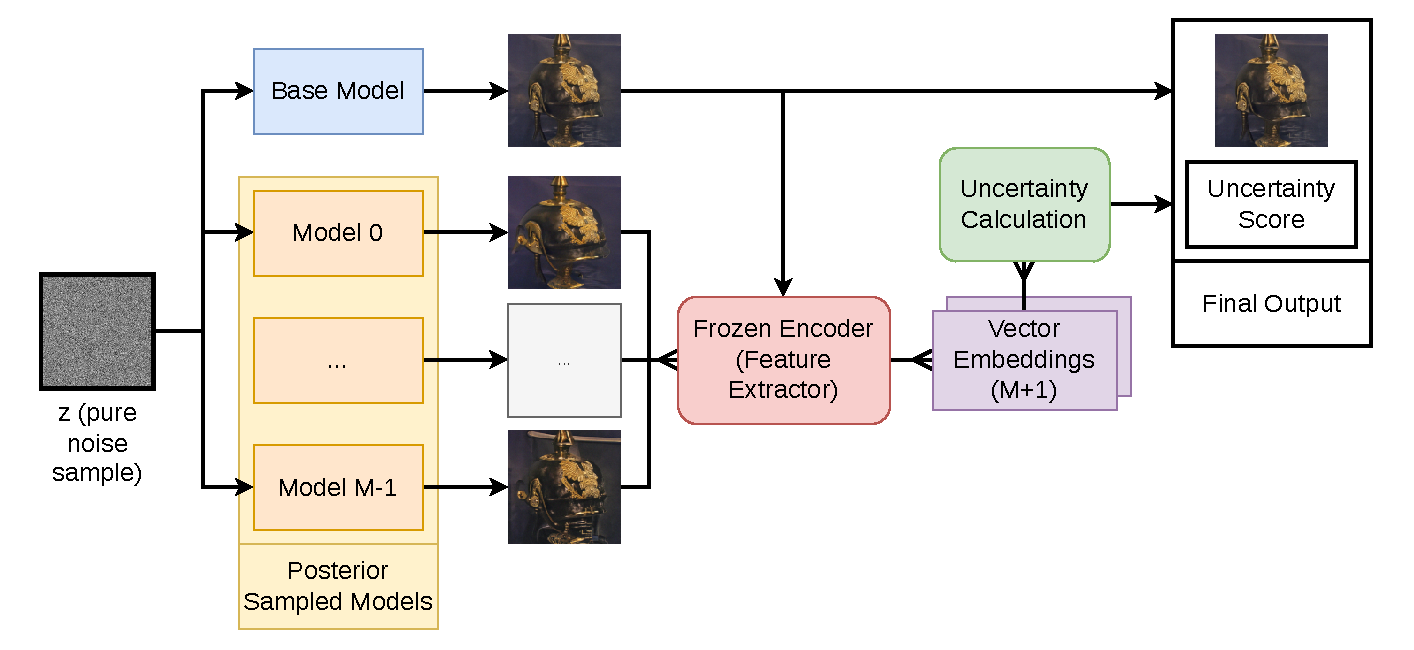
\includegraphics[width=0.9\linewidth]{figures/gu_theory/uncertainty_pipeline.pdf}
    \caption{Pipeline mapping the progression from the Posterior Approximation to the Semantic Vectors used for uncertainty computation.}
    \label{fig:pipeline_posterior_to_vector}
\end{figure}


\autoref{fig:pipeline_posterior_to_vector} outlines the uncertainty computation pipeline. 
\begin{enumerate}
    \item First, we form a \acs{LA} posterior $q(\theta|\mathcal{D})$ centered around the base model $\hat\theta$. Then we sample M models $\boldsymbol{\theta} \sim q(\theta|\mathcal{D})$ from that posterior.
    \item We are now ready to generate images. We sample a single, fixed noise sample $z \sim \mathcal{N}(0,I)$ that we feed through the base model as well as the M sampled models (everyone gets the same noise sample). This gives us $M+1$ generated images that only differ by the model weights used. 
    \item We pass those $\mathrm{M}+1$ generated images through a semantic encoder (feature extractor) to get $\mathrm{M}+1$ vector embeddings.
    \item We compute the uncertainty by fitting a Gaussian distribution on those $\mathrm{M}+1$ vectors and computing its entropy.
\end{enumerate}

\begin{tcolorbox}[colback=gray!10!white,colframe=gray!50!black,sharp corners]
The intuition here is ``\textit{if a small perturbation in the models weights changes the meaning of image drastically, the model is highly uncertain about its output and should assign it a high uncertainty}''.
\end{tcolorbox}

\section{Bayesian Model}
\label{sec:bayesian_model}

In this section, we formalize the definition of the posterior predictive distribution in both image and semantic vector space which is later used to compute the uncertainty. 

\begin{tcolorbox}[colback=blue!10!white,colframe=blue!50!black,sharp corners]
Because we are not yet trying to compute the uncertainty, in this section we will only define the full continuous form of the posterior predictive distribution which will later be approximated with the Monte Carlo \acs{MC} method to make the uncertainty computation feasible (\autoref{sec:bg_gu_uncertainty_computation_mc}).
\end{tcolorbox}

We first describe how \cite{jazbec_generative_2025} modeled their method mathematically. Then we highlight theoretical issues in their formulation and offer a mathematical re-framing that partially restores the rigor needed by the Bayesian framework. Doing so will expose the real, previously hidden theoretical issues of their method.

% \begin{tcolorbox}[colback=blue!10!white,colframe=blue!50!black,title=Pipeline Overview,sharp corners]
% Because we are analyzing the theoretical posterior predictive distribution, we focus here on its continuous (integral) formulation. The pipeline overview in \autoref{sec:pipeline_overview} already accounts for the Monte Carlo approximation of this formulation.
% \end{tcolorbox}

\subsection{The Formulation by \cite{jazbec_generative_2025}}

To quantify generative uncertainty in diffusion models, \parencite{jazbec_generative_2025} propose a post-hoc Bayesian framework. Their objective is to capture the model's epistemic uncertainty by placing a distribution over the pre-trained neural network weights and propagating that uncertainty to the final generated images.

\paragraph{The Proposed Pipeline}
Their methodology can be broken down into three core components:

\begin{enumerate}
    \item \textbf{Empirical Parameter Posterior:} They approximate the posterior distribution over the model weights $q(\theta | \mathcal{D})$ using a Laplace approximation centered on the pre-trained base model weights, $\hat{\theta}$. 
    
    % The covariance matrix $\Sigma_\theta$ relies on the Hessian of the standard unweighted diffusion loss, $\mathcal{L}_{\mathrm{simple}}(\theta)$. 
    % To complete the Bayesian formulation, they adopt an isotropic Gaussian prior $p(\theta) = \mathcal{N}(\theta; 0, \gamma^{-1}I)$, which mathematically introduces a prior precision term $\gamma I$ into the inverse Hessian computation:

    To get the Hessian expression, we start from \autoref{eq:hessian_joint} and make the following assumptions:
    \begin{itemize}
        \item The simple loss $\mathcal{L}_{\mathrm{simple}}$ is equivalent to the negative log likelihood $-\log p(\mathcal{D}|\theta)$
        \item The prior is an isotropic Gaussian $p(\theta) = \mathcal{N}(\theta; 0, \gamma^{-1}I)$. (For which the Hessian is equal to $\gamma I$.)
    \end{itemize}
    And we get the following expression:
    
    \begin{align}
    H &= -\nabla^2_\theta \log p(\mathcal{D}|\theta)|_{\theta=\hat\theta} -\nabla^2_\theta \log p(\theta)|_{\theta=\hat\theta}\\
    &= \nabla_{\theta}^{2}\mathcal{L}_{\mathrm{simple}}(\theta)|_{\hat{\theta}} + \gamma I \label{eq:jazbec_laplace}
    \end{align}
    Which gives us the \acs{LA} posterior approximation 
    \begin{align}
    q(\theta | \mathcal{D}) = \mathcal{N}(\theta; \hat{\theta}, H^{-1}) = \mathcal{N}(\theta;\hat\theta,\Sigma_\theta)
    \end{align}
    
    (Note: While \cite{jazbec_generative_2025} omit the $\gamma I$ term in their main text formulation, they explicitly use this prior in their implementation details).

    \item \textbf{Deterministic Semantic Generation:} To isolate the model's epistemic uncertainty from the inherent stochasticity of the generative process, they rely on a deterministic generation path\footnote{\acs{DDPM} models can be made deterministic by fixing the noise seed used throughout the reverse diffusion process. For \acs{DDIM}, the process is already inherently deterministic.}. A fixed initial noise sample $z \sim \mathcal{N}(0, I)$ is injected through the unrolled reverse sampler $g_\theta(z)$ to output a generated image $x$. Furthermore, to prevent the uncertainty metric from being affected by irrelevant, pixel-level background noise, they project the generated image through a pretrained semantic encoder $c_\phi : \mathbb{R}^D \rightarrow \mathbb{R}^K$ into a semantic vector space. This defines the deterministic semantic generator: $S(\theta) = c_\phi(g_\theta(z))$.

    \item \textbf{Semantic Predictive Posterior:} Finally, defining $e = c_\phi(x)$ as the semantic feature vector and $\sigma^2$ as the observation noise variance, the predictive posterior is obtained by marginalizing over the approximate parameter posterior:
    \begin{align}
        p(e | z, \theta) &= \mathcal{N}\left(e; S(\theta), \sigma^2 I\right)\\
        % p(e | z, \mathcal{D}) &= \int p(e | z, \theta) p(\theta | \mathcal{D}) d\theta \\
        p(e | z, \mathcal{D}) &\overset{LA}{\simeq} \int p(e | z, \theta) q(\theta | \mathcal{D}) d\theta \\
        &= \int \mathcal{N}\left(e; S(\theta), \sigma^2 I\right) \mathcal{N}\left(\theta; \hat{\theta}, \Sigma_\theta\right) d\theta \nonumber
    \end{align}
\end{enumerate}

\paragraph{The Theoretical Issues}
As acknowledged by \cite{jazbec_generative_2025}, this formulation is theoretically flawed when viewed through a strict Bayesian lens. 

Properly applying the Laplace approximation to the posterior $p(\theta|\mathcal{D})$ requires the loss function to be equivalent to the negative log of the joint distribution $-\log p(\theta, \mathcal{D})$, which encompasses both the exact data log-likelihood and a prior term. The framework by \cite{jazbec_generative_2025} falls short on both fronts:

The unweighted \acs{MSE} objective $\mathcal{L}_{\mathrm{simple}}(\theta)$ is not equivalent to the negative log joint distribution $-\log p (\theta, \mathcal{D})$ nor is it equivalent to the negative log likelihood $-\log p(\mathcal{D}|\theta)$.

\begin{enumerate}
    \item $\mathcal{L}_{\mathrm{simple}} \not\equiv -\log p(\mathcal{D}|\theta)$. As we have seen in \autoref{sec:bg_diffusion}, $\mathcal{L}_{\mathrm{simple}}$ was obtained by dropping the timestep dependent weights from the loss derived from the theory. $\mathcal{L}_{\mathrm{simple}}$ can therefore not be used as a surrogate for the likelihood for the whole reverse diffusion process. \label{enum:l_simple}
    \item $\mathcal{L}_{\mathrm{weighted}} \not \equiv -\log p(\theta, \mathcal{D})$. As we have seen in \autoref{sec:bg_laplace}, The diffusion models we use here are trained to find the \acs{MLE}. So even if we use the proper weighted loss, we would only have it be a proper surrogate of the negative log likelihood $-\log p(\mathcal{D}|\theta)$ and not the full joint distribution. \label{enum:l_weighted}
\end{enumerate}

\ref{enum:l_simple} will be addressed by changing our perspective from image data to intermediate noise prediction. However, \ref{enum:l_weighted} is a fundamental flaw of how the base model was trained, and the whole point of this method is to not retrain the model, we kept it as it is and considered $\gamma$ to be a regularization constant for the Hessian inversion.

% \begin{itemize}
%     \item \textbf{The Likelihood Discrepancy:} The unweighted \acs{MSE} objective $\mathcal{L}_{\mathrm{simple}}(\theta)$ is not mathematically equivalent to the true log-likelihood of the image data $\mathcal{D}$. As acknowledged by the authors, obtaining the true data likelihood would require a specific, complex timestep-dependent weighting scheme.
%     \item \textbf{The Prior Discrepancy (\acs{MLE} vs. \acs{MAP}):} Because standard diffusion training lacks explicit probabilistic prior regularization, the pre-trained weights $\hat{\theta}$ represent a Maximum Likelihood Estimate (\acs{MLE}), not the Maximum A Posteriori (\acs{MAP}) estimate required for a strict Laplace expansion. The prior term $\gamma I$ in Equation \ref{eq:jazbec_laplace} is not an intrinsic part of the training objective; it is a post-hoc surrogate added solely to stabilize the matrix inversion.
% \end{itemize}

% Consequently, while the covariance matrix $\Sigma_\theta$ effectively captures the curvature of the $\mathcal{L}_{\mathrm{simple}}$ optimization landscape, it lacks a rigorous Bayesian interpretation relative to the original training data $\mathcal{D}$.

\subsection{An Alternative Model Using Exact Likelihood}

We can resolve inconsistency \ref{enum:l_simple} by shifting our perspective on the likelihood. Rather than forcing $\mathcal{L}_{\mathrm{simple}}$ to represent the log-likelihood of the image data $\mathcal{D}$, we frame it around the model's actual training task: predicting the added noise.

By defining an effective dataset of noise-prediction tasks $\mathcal{D}_{noise} = \{(x_{t,i}, t_i, \epsilon_i)\}_{i=1}^N$ (where at $t_i$, $x_{t,i}$ is the intermediate noisy image and $\epsilon_i$ the intermediate noise added to the image), we transform the formulation into an exact Bayesian regression problem. The likelihood of observing this whole effective dataset becomes:

\begin{align}
    p(\mathcal{D}_{noise} | \theta) &= \prod_{i=1}^N p(x_{t,i}, t_i, \epsilon_i | \theta)
\end{align}

We can then reformulate this using Bayes' rule:
\begin{align}
    p(x_{t,i}, t_i, \epsilon_i | \theta) &= p(\epsilon_i | x_{t,i}, t_i, \theta) \cdot p(x_{t,i}, t_i | \theta)
\end{align}

Making the reasonable assumption that $\theta$ has no influence on how timesteps $t_i$ are sampled and how the forward diffusion process creates $x_{t,i}$, we can simplify $p(x_{t,i}, t_i | \theta) = p(x_{t,i}, t_i)$ and the likelihood becomes:
\begin{align}
    p(\mathcal{D}_{noise} | \theta) &= \prod_{i=1}^N p(\epsilon_i | x_{t,i}, t_i, \theta) \cdot p(x_{t,i}, t_i)
\end{align}

Since we are optimizing $\theta$ when training, anything that's independent of $\theta$ can be viewed as constant. This leaves us with this expression for the \acs{NLL} (negative log likelihood).

\begin{align}
-\log p(\mathcal{D}_{noise} | \theta) = \sum_{i=1}^N -\log p(\epsilon_i | x_{t,i}, t_i, \theta) + C \label{eq:general_noise_likelihood}
\end{align}

For this \acs{NLL} to reduce to $\mathcal{L}_{\mathrm{simple}}$ (up to normalization), we define:
\begin{align}
    p(\epsilon_i | x_{t,i}, t_i, \theta) &= \mathcal{N}\left(\epsilon_i; \epsilon_\theta(x_{t,i}, t_i), s^2 I\right) \label{eq:noise_likelihood}
\end{align}

To fix inconsistency \ref{enum:l_simple}, we only need to show the equivalence between $\mathcal{L}_{\mathrm{simple}}$ and the negative log likelihood $-\log p(\mathcal{D}_{noise}|\theta)$ rather than with the full negative log joint distribution $- \log p(\theta,\mathcal{D})$.

% With this framing of the likelihood, we can indeed prove that 
% \begin{align}
% -\log p(\mathcal{D}_{noise}|\theta) = \mathcal{L}_{\mathrm{simple}} + C
% \end{align}
% See \autoref{app:l_simple_nll_equivalence} for the full proof.

To show this, we start from \eqref{eq:noise_likelihood}:
\begin{align}
p(\epsilon_i | x_{t,i}, t_i, \theta) &= \frac{1}{\sqrt{(2\pi s^2)^D}} \exp\left( - \frac{1}{2s^2} ||\epsilon_i - \epsilon_\theta(x_{t,i}, t_i)||_2^2 \right) \nonumber \\
-\log p(\epsilon_i | x_{t,i}, t_i, \theta) &= \underbrace{-\log\left( \frac{1}{\sqrt{(2\pi s^2)^D}} \right)}_{c \indep \theta} + \frac{1}{2s^2} ||\epsilon_i - \epsilon_\theta(x_{t,i}, t_i)||_2^2 \nonumber
\end{align}

Grouping the part that's independent of $\theta$ in $c$ and setting $s^2 = 1/2$ allows us to get the exact expression of a term from the simplified loss (\acs{MSE}).

\begin{equation}
-\log p (\epsilon_i | x_{t,i}, t_i, \theta) = ||\epsilon_i - \epsilon_\theta(x_{t,i}, t_i)||_2^2 + c \label{eq:noise_loss_single_lik}
\end{equation}

Which leads to the \acs{NLL}, by injecting \autoref{eq:noise_loss_single_lik} in \autoref{eq:general_noise_likelihood}:
\begin{align}
    - \log p(\mathcal{D}_{noise}|\theta) &= \sum^N_{i=1} - \log p(\epsilon_i|x_{t,i},t_i,\theta) + C\\
    &= \sum^N_{i=1} ||\epsilon_i - \epsilon_\theta(x_{t,i}, t_i)||_2^2 + C'\\
    &= N\,\mathcal{L}_{\mathrm{simple}} + C' \label{eq:nll_n_lsimple}
\end{align}

Here $C, C'$ collect everything that is constant w.r.t. $\theta$. The factor $N$ simply reflects the difference between a mean and a sum: $\mathcal{L}_{\mathrm{simple}}$ is defined in the literature as a per-sample \emph{expectation} \eqref{eq:simple_loss} (estimated by the empirical mean over the $N$ noise-prediction samples), whereas the dataset negative log-likelihood is the corresponding \emph{sum} over those samples. We keep $\mathcal{L}_{\mathrm{simple}}$ exactly as defined in \cite{ho_denoising_2020}; the constant $N$ is independent of $\theta$, so it leaves the trained minimizer $\hat\theta$ unchanged. It is, however, the genuine scale of the data likelihood, and it stays in the likelihood term: the Laplace Hessian is the curvature of the full (summed) negative log-likelihood,
\begin{equation}
\nabla^2_\theta\left[-\log p(\mathcal{D}_{noise}|\theta)\right]\big|_{\hat\theta} = N\,\nabla^2_\theta\,\mathcal{L}_{\mathrm{simple}}(\theta)\big|_{\hat\theta},
\label{eq:nll_hessian_scale}
\end{equation}
which we estimate with the empirical Fisher accumulated over the dataset (\autoref{sec:bg_gu_further_approx}). 
% The isotropic Gaussian prior then contributes its precision $\gamma I$ on top (\autoref{sub:la_trained_on_mle}) as a genuine prior. This repairs the broken link of issue \ref{enum:l_simple}.

% Under the assumption of a uniform prior (effectively making \acs{MLE} $=$ \acs{MAP}), we can prove that the negative log-likelihood perfectly equates to the diffusion loss: $$-\log(p(\mathcal{D}_{noise}|\theta)p(\theta)) = \mathcal{L}_{\mathrm{simple}} + C$$ (detailed in ). This shift ensures that the loss function evaluated for the Laplace approximation's Hessian is mathematically identical to the exact negative log-likelihood.

% The updated parameter posterior and semantic predictive posterior become:
% \begin{align}
%     p(\theta | \mathcal{D}_{noise}) &\simeq q(\theta | \mathcal{D}_{noise}) = \mathcal{N}\left(\theta; \hat{\theta}, \Sigma_\theta\right) \\
%     p(e | z, \theta) &= \mathcal{N}\left(e; S(\theta), \sigma^2 I\right)\\
%     p(e | z, \mathcal{D}_{noise}) &= \int p(e|z, \theta)p(\theta|\mathcal{D}_{noise})d\theta \\
%     &\simeq \int \mathcal{N}\left(e; S(\theta), \sigma^2 I\right) \mathcal{N}\left(\theta; \hat{\theta}, \Sigma_\theta\right) d\theta
% \end{align}
The semantic predictive posterior remains the same as before:
\begin{align}
        p(e | z, \mathcal{D}) &\simeq \int \mathcal{N}\left(e; S(\theta), \sigma^2 I\right) \mathcal{N}\left(\theta; \hat{\theta}, \Sigma_\theta\right) d\theta \label{eq:semantic_post_pred}
\end{align}

But now, $\Sigma_\theta = H^{-1}$ is theoretically grounded w.r.t. theoretical issue \ref{enum:l_simple}. From here on we use $\mathcal{D}$ and $\mathcal{D}_{noise}$ interchangeably when conditioning the posterior, since the \acs{LA} is now grounded on the noise-prediction likelihood $p(\mathcal{D}_{noise}|\theta)$.

% is properly derived from the Empirical Fisher Information matrix of the noise-prediction negative log-likelihood, evaluated at the \acs{MLE} $\hat{\theta}$.

% \subsection{Prior and MAP Estimator}
% \label{sub:mle_map_eq}

% Evaluating the Laplace approximation at $\hat{\theta}$ relies on an \acs{MLE} obtained from standard training. A true \acs{MAP} estimate requires optimizing the joint probability $p(\theta, \mathcal{D}_{noise})$, which occurs naturally if the network is trained with L2 regularization (e.g., \texttt{AdamW} weight decay). Because models like ADM typically omit this, we manually introduce a post-training prior $\gamma$ to prevent division by zero in the inverse Hessian computation.

% While assuming an infinitely flat prior would mathematically force $\acs{MLE} = \acs{MAP}$, it is numerically unstable. Fortunately, the approximation $\acs{MLE} \simeq \acs{MAP}$ holds in practice because the massive scale of the data likelihood vastly dominates the prior term. Following the empirical validation in \parencite[Appendix D]{jazbec_generative_2025}, we set $\gamma = 1.0$, which optimally balances computational stability with metric performance (FID, precision, and recall).

\subsection{New Theoretical Issues}

Aligning the likelihood with the target noise exposes two theoretical issues that were previously hidden in the incomplete \cite{jazbec_generative_2025} Bayesian framework:

\begin{enumerate}
    \item \textbf{IID Violation:} Viewing the training dataset as the original data $\mathcal{D}$ enriched with intermediate noisy states means multiple samples originate from the same clean image, potentially violating the Independent and Identically Distributed (\acs{IID}) assumption. \label{enum:iid_violation}
    \item \textbf{Multi-Step Inference:} The \acs{LA} is computed on a single-step denoiser $\epsilon_\theta$. Theoretically, uncertainty should be measured over a single step. In practice, however, we use the \acs{LA} to sample network weights, run the full multi-step reverse process, and measure uncertainty only at the final step $t=0$. \label{enum:multi-step-inference}
\end{enumerate}

Issue \ref{enum:iid_violation} is more of an open question that we did not have an answer to. 
Issue \ref{enum:multi-step-inference} however will be discussed in depth now.

\subsection{Multi-Step Inference in Bayesian Framework}
\label{sub:gu_theory_issue_multi_step}

\cite{jazbec_generative_2025} was based on \cite{kou_bayesdiff_2024}. Two main contributions were made by \cite{jazbec_generative_2025}. The first one was adding a pre-trained (external) semantic encoder to evaluate uncertainty in its latent space rather than in pixel-space. The second was to only evaluate uncertainty on the last step of the reverse diffusion process (final image output). The second being a direct consequence of the first one because the external encoder is not made to process noisy images.

While it is true that a proper Bayesian framework should track uncertainty across all reverse diffusion timesteps, We show much later in the thesis (\autoref{ch:using_internal_encoder}, using an internal encoder that understands intermediate noisy images in the reverse diffusion process) that the final generated image $x_0$ is the best timestep at which to extract the uncertainty if it's used to filter for visual quality. 
So from a pure performance standpoint, it seems we can rely on tracking uncertainty in the final timestep $t=0$ only.

\cite{gupta_quantifying_2026} (FLARE) also argue that not tracking uncertainty across all reverse diffusion timesteps prevents us from properly separating epistemic uncertainty\footnote{Uncertainty in the model's knowledge} from aleatoric uncertainty\footnote{Uncertainty stemming from inherent noise in the reverse diffusion process and data}. We argue however that fixing a noise seed for both the starting noise $z$ and stochastic noise injection for \acs{DDPM}s allows us to properly isolate epistemic uncertainty.

% \subsection{FLARE Framework}

% \cite{gupta_quantifying_2026} address this multi-step discrepancy by analytically propagating epistemic uncertainty through the entire Markov chain within the single-step denoiser space. However, computing the necessary backward steps for the Jacobian significantly increases computational cost and implementation complexity.

%%%%%%%%%

\section{Uncertainty Computation}
\label{sec:bg_gu_uncertainty_computation_mc}

In this section, we define the mathematical framework to compute the generative uncertainty starting from the semantic posterior predictive \autoref{eq:semantic_post_pred}. In parallel, we will also describe the approximations made along the way.

The first step is to compute the semantic posterior predictive:
\begin{align}
p(e | z, \mathcal{D}_{noise}) &\overset{LA}{\simeq} \int p(e|z,\theta) q(\theta|\mathcal{D}_{noise}) d\theta \\
&= \mathbb{E}_{q(\theta|\mathcal{D}_{noise})}\left[p(e|z,\theta)\right]
\end{align}
Clearly, this integral is intractable. A simple method to go around this limitation is using a Monte Carlo approximation. And the integral becomes
\begin{align}
\mathbb{E}_{q(\theta|\mathcal{D}_{noise})}\left[p(e|z,\theta)\right] &\overset{MC}{\simeq} \frac{1}{\mathrm{M}+1} \sum^\mathrm{M}_{m=0}p(e|z,\theta_m)\\ 
&=\frac{1}{\mathrm{M}+1} \sum^\mathrm{M}_{m=0} \mathcal{N}(e;S(\theta_m), \sigma^2 I)
\end{align}

With $\theta_m \sim q(\theta|\mathcal{D}_{noise})$. We then approximate this mixture of Gaussians as a single Gaussian $\mathcal{N}(e|\mu^*,\Sigma^*)$ using moment matching. We first define $e_m = S(\theta_m)$ and then compute the moments:
\begin{itemize}
    \item First moment (matching the mean): $\mu^* = \frac{1}{\mathrm{M}+1} \sum^{\mathrm{M}}_{m=0} e_m$
    \item Second moment (matching the covariance) (by the law of total variance):
    \begin{align}
    \Sigma^* &= \sigma^2 I + \frac{1}{\mathrm{M}+1} \sum^\mathrm{M}_{m=0} e_m e_m^\top - \mu^*(\mu^*)^\top
    \end{align}
\end{itemize}

For efficiency reasons, we only consider the diagonal terms of $\Sigma^*$:
\begin{align}
    \Sigma^* &\simeq \sigma^2 I + \text{Diag}\left(\frac{1}{\mathrm{M}+1}\sum^\mathrm{M}_{m=0} e_m e_m^\top - \mu^*(\mu^*)^\top \right) =: \Sigma^{d*}
\end{align}

In the end, we get $p(e|z,\mathcal{D}) \simeq \mathcal{N}(e;\mu^*,\Sigma^{d*})$. The generative uncertainty is defined as the entropy of this distribution: $\mathcal{U}(x)$.
The diagonal covariance matrix $\Sigma^{d*}$ is in $\mathbb{R}^{K\times K}$; we define $\sigma_k^2$ as its $k$-th diagonal element (i.e.\ the variance of the $k$-th semantic dimension) and the uncertainty is defined as:

\begin{equation}
\mathcal{U}(x) = \frac{1}{2} \sum_{k=1}^K \ln(\sigma_{k}^2) + const
\end{equation}

As a side note, this Monte Carlo approximation of the bayesian posterior objective using a finite ensemble of models makes other non-Bayesian methods integrate seamlessly in our framework. For instance, in the \textit{Toy Experiment} we first use a Deep Ensemble (\acs{DE}) of models which is obtained by training multiple models with different random seeds.

\section{Further Approximation Considerations}
\label{sec:bg_gu_further_approx}

Although we've defined the \acs{LA}, we've yet to detail how we can compute $H$, the Hessian matrix of the negative log-posterior evaluated at the mode $\hat\theta$.

\begin{equation}
    H = -\nabla_\theta^2 \log p(\mathcal{D}_{noise}|\theta)|_{\theta=\hat\theta} + \gamma I
\end{equation}

This matrix captures the geometric curvature of the loss landscape, where the inverse of this curvature ($H^{-1}$) dictates the model's epistemic uncertainty (the covariance matrix $\Sigma_{\theta}$).  

$H$ consists of two parts: the Hessian of the negative log likelihood (\acs{NLL}) and the Hessian of the negative log prior. 

For a neural network with $P$ parameters, the exact Hessian matrix of the \acs{NLL} $H_{\mathrm{NLL}}\in \mathbb{R}^{P \times P}$ scales quadratically. For modern architectures with millions of weights, computing, storing, and later inverting the dense matrix $H$ is almost impossible.

To make the computation tractable, \cite{jazbec_generative_2025} approximate the curvature using the empirical Fisher Information Matrix (\acs{FIM}).

Mathematically, the empirical \acs{FIM} ($\hat{F}$) approximates the expected Hessian of the negative log likelihood using first-order gradients (which are vastly cheaper to compute than second-order derivatives). For $N$ data points, the empirical FIM is defined as:

\begin{align}
\hat{F} = \frac{1}{N} \sum_{i=1}^N \nabla_{\theta} \log p(\epsilon_i|x_{t,i}, t_i,\theta) \nabla_{\theta} \log p(\epsilon_i|x_{t,i}, t_i,\theta)^T 
\end{align}

This still gives us a $P\times P$ sized matrix. In \cite{jazbec_generative_2025} we further approximate the empirical \acs{FIM} by only keeping the diagonal terms, giving us $P$ elements.

\begin{equation}
\hat{F}_{pp} = \frac{1}{N} \sum_{i=1}^N \left( \frac{\partial \log p(\epsilon_i|x_{t,i},t_i, \theta)}{\partial \theta_p} \right)^2
\end{equation}

In the end, we get
\begin{equation}
H \simeq N\,\mathrm{Diag}(\hat{F}) + \gamma I.
\end{equation}
The factor $N$ converts the per-sample averaged Fisher $\hat F$ into the curvature of the full-dataset negative log-likelihood (\autoref{eq:nll_hessian_scale}); equivalently, $N\hat F$ is just the empirical Fisher \emph{summed} over the $N$ samples rather than averaged. The prior precision $\gamma$ is added on top: because the data term scales with $N$ while the prior does not, $\gamma$ is small relative to the likelihood curvature, which is exactly the regime in which the \acs{MLE}~$\simeq$~\acs{MAP} approximation of \autoref{sub:la_trained_on_mle} would be justified.

To further reduce $P$, instead of using a \acs{LA} over the full network, \cite{jazbec_generative_2025} restricts the approximation to the last layer of the network $=:$ Last Layer Laplace Approximation \acs{LLLA}.

\begin{tcolorbox}[colback=orange!10!white,colframe=orange!50!black,sharp corners]
\cite{gupta_quantifying_2026} heavily criticizes the \acs{LLLA} and suggests instead a random subnetwork Laplace approximation with a full covariance matrix. They argue that it is preferable to have a posterior approximation that samples fewer parameters than the \acs{LLLA} but spreads them across more layers and uses a full covariance matrix to preserve the interactions between parameters.

In \autoref{ch:toy_exp_posterior}, we still show that despite the criticism, the \acs{LLLA} can be a very capable approximation to filter \acs{OOD} samples for a Toy model.
\end{tcolorbox}

Finally, to reduce the time needed to compute $\hat{F}$ even further, (\cite{jazbec_generative_2025}, Appendix D) use only $1\%$ of the training data for the \acs{ADM} (the \textit{Toy Model} will use the full training set).

\begin{tcolorbox}[colback=orange!10!white,colframe=orange!50!black,sharp corners]
As a side note, \emph{if} the empirical Fisher is accumulated as a sum over training samples (as the reference implementation \parencite{jazbec_generative_2025} appears to do), the negative-log-likelihood term of the Hessian scales with $N$ (\autoref{eq:nll_hessian_scale}). Computing the empirical Fisher on only $1\%$ of the data would then affect the posterior covariance matrix $\Sigma_\theta = H^{-1}$ in a way that can increase the spread of the gaussian weight posterior distribution. The effect of playing with the scale of the covariance matrix is investigated on the \textit{Toy Experiment} in \autoref{ch:toy_exp_posterior}. It is however much harder to investigate on the \acs{ADM} because of the semantic encoder possibly hides any improvement to the posterior approximation (\autoref{ch:semantic-encoder}).
\end{tcolorbox}

\subsection{Toy Model Posterior Approximation}
\label{sub:gu_th_toy_model_posterior_approximation}

Chapters \ref{ch:reproduce_toy}, \ref{ch:quantifying_gu_filtering_toy}, \ref{ch:toy_exp_posterior} use the much smaller diffusion \textit{Toy Model} that works with $x \in \mathbb{R}^2$. 

The size of the Toy Model is small enough to allow the training of multiple independent models giving us a Deep Ensemble (\acs{DE}) that will be compared to an \acs{LLLA} Sampled Ensemble (as used for the \acs{ADM}).

Additionally, because the Toy Model output space is only 2D, we don't need to use a semantic encoder to compute the uncertainty. 

% In \autoref{ch:toy_exp_posterior}, we will show

% this result will come in handy when we later discover that the semantic encoder can be used without the bayesian framework to compute uncertainty (\autoref{ch:semantic-encoder}).